\documentclass[10pt,twocolumn,letterpaper]{article}

\usepackage{cvpr}
\usepackage{times}
\usepackage{epsfig}
\usepackage{graphicx}
\usepackage{amsmath}
\usepackage{amssymb}
\usepackage{float}

% Include other packages here, before hyperref.

% If you comment hyperref and then uncomment it, you should delete
% egpaper.aux before re-running latex.  (Or just hit 'q' on the first latex
% run, let it finish, and you should be clear).
\usepackage[breaklinks=true,bookmarks=false]{hyperref}

\cvprfinalcopy % *** Uncomment this line for the final submission

\def\cvprPaperID{****} % *** Enter the CVPR Paper ID here
\def\httilde{\mbox{\tt\raisebox{-.5ex}{\symbol{126}}}}

% Pages are numbered in submission mode, and unnumbered in camera-ready
%\ifcvprfinal\pagestyle{empty}\fi
\setcounter{page}{1}
\begin{document}

%%%%%%%%% TITLE
\title{Translating an electrical circuit schematic into a SIMULINK model}

\author{Andreas Boltres\\
Karlsruhe Institute of Technology\\
Kaiserstr. 12, 76131 Karlsruhe, Germany\\
{\tt\small andreas.boltres@student.kit.edu}
% For a paper whose authors are all at the same institution,
% omit the following lines up until the closing ``}''.
% Additional authors and addresses can be added with ``\and'',
% just like the second author.
% To save space, use either the email address or home page, not both
\and
Cem G\"ul\c{s}an\\
Hamburg University of Technology\\
Am Schwarzenberg-Campus 1, 21073 Hamburg, Germany\\
{\tt\small cem.guelsan@tuhh.de}
\and
Christian Alexander Vecsei\\
RWTH Aachen\\
Templergraben 55, 52062 Aachen, Germany\\
{\tt\small christian.vecsei@rwth-aachen.de}
\and
Thomas Frei\\
University of Applied Sciences and Arts Northwestern Switzerland\\
Bahnhofstrasse 6, 5210 Windisch, Switzerland\\
{\tt\small thomas.frei1@students.fhnw.ch}
}

\maketitle

% ABSTRACT-------------------

\begin{abstract}
We present a functionality developed within the computing environment MATLAB, which analyses schematics of electrical circuits and transforms them into an electrical circuit model of MATLAB's SIMULINK environment.
\end{abstract}

% INTRO---------------------------------------------------------

\section{Introduction}
\label{sec:intro}

\subsection{Motivation}
\label{subsec:moti}

Students and engineers often use schematics while studying or developing. A schematic is a drawing of an electric circuit which should contain all information about the circuit but should also be as simple as possible.
\par
With increasing size, electrical circuits often become more complicated and confuse less experienced engineers, rendering the estimation of the circuit's behaviour hard or impossible.
\par

\begin{figure}[!ht]
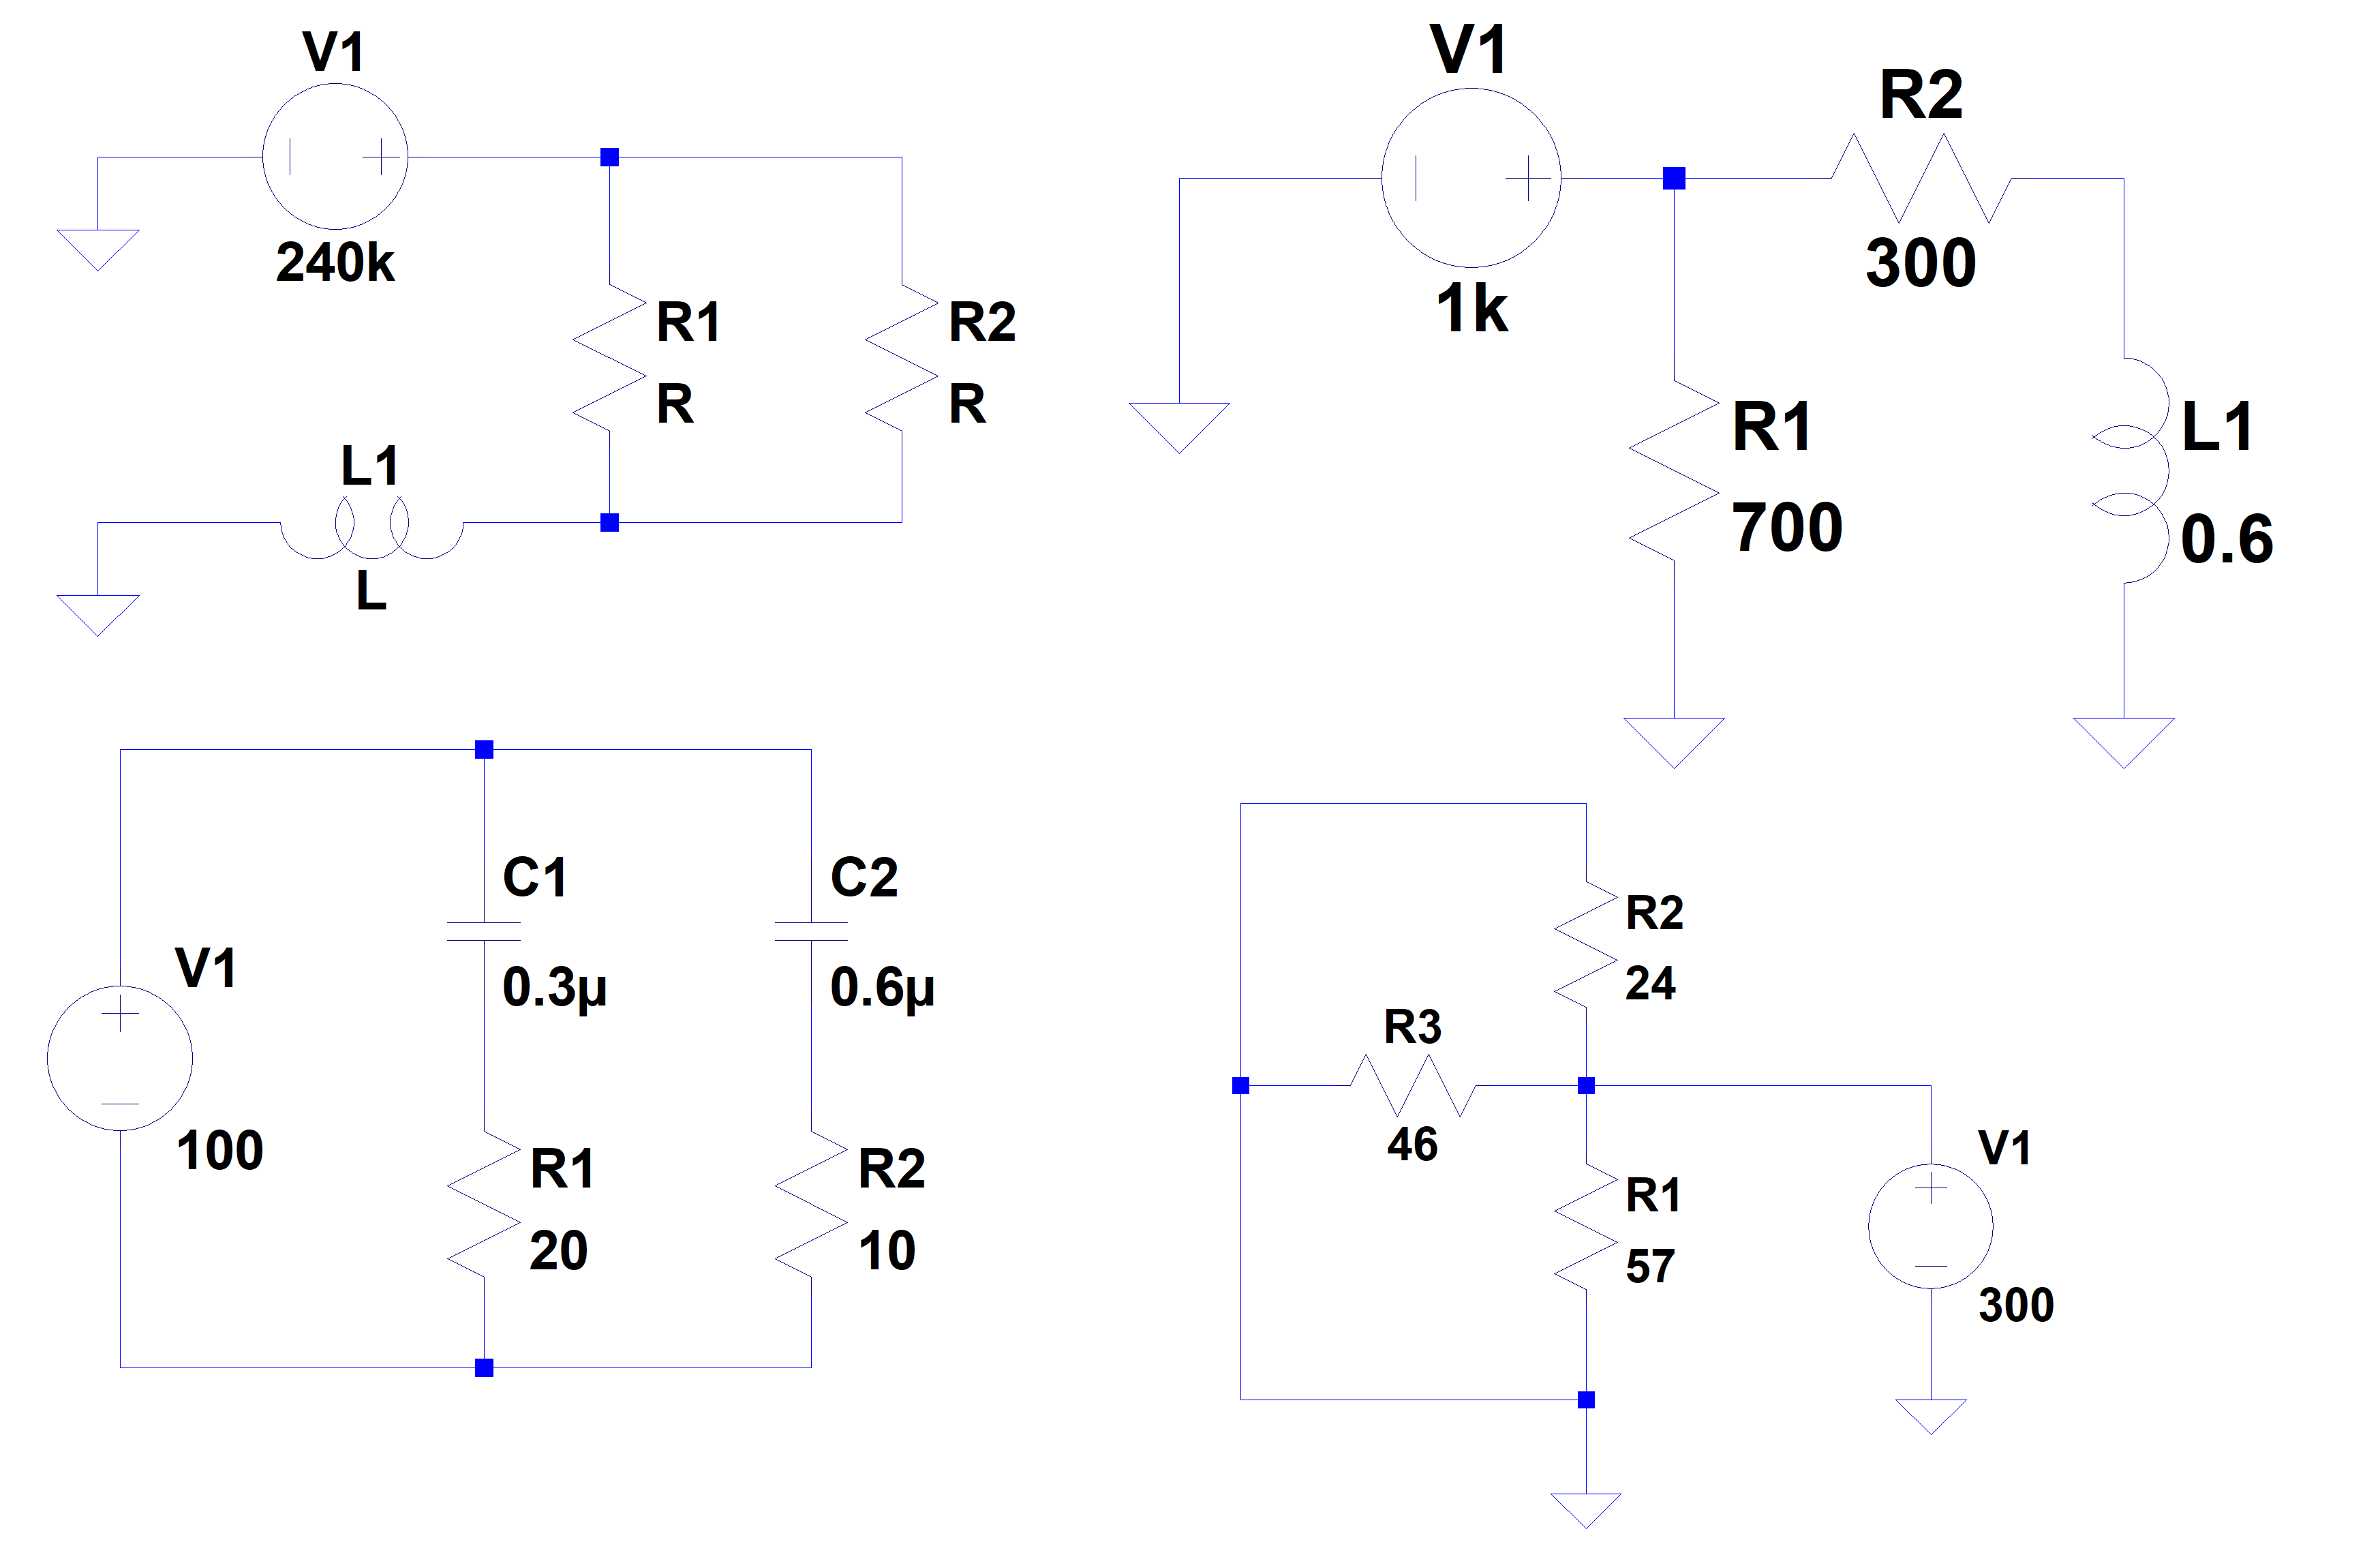
\includegraphics[width = 3.2in]{img/circuits.png}
\caption{Example circuits}
\label{fig:c1}
\end{figure}

\par
A program that confidently identifies the components of a schematic with their respective connections and translates them into a user-friendly digital model can substantially accelerate the understanding of the given circuit. Analyzing, modifying and storing a schematic becomes easy once it is properly digitized.

\subsection{Program overview}
\label{subsec:over}

The aim of this student project is, as stated in the abstract, to create a functionality developed within the computing environment MATLAB, analyzing schematics of electrical circuits and transforming them into an electrical circuit model within MATLAB's Simulink environment. There, it can be used to facilitate calculations or behaviour analyses. The process of obtaining the Simulink model from the given image can be divided into three phases which will be briefly described in the following sentences and in detail in the following sections.
\par

\begin{figure}[!ht]
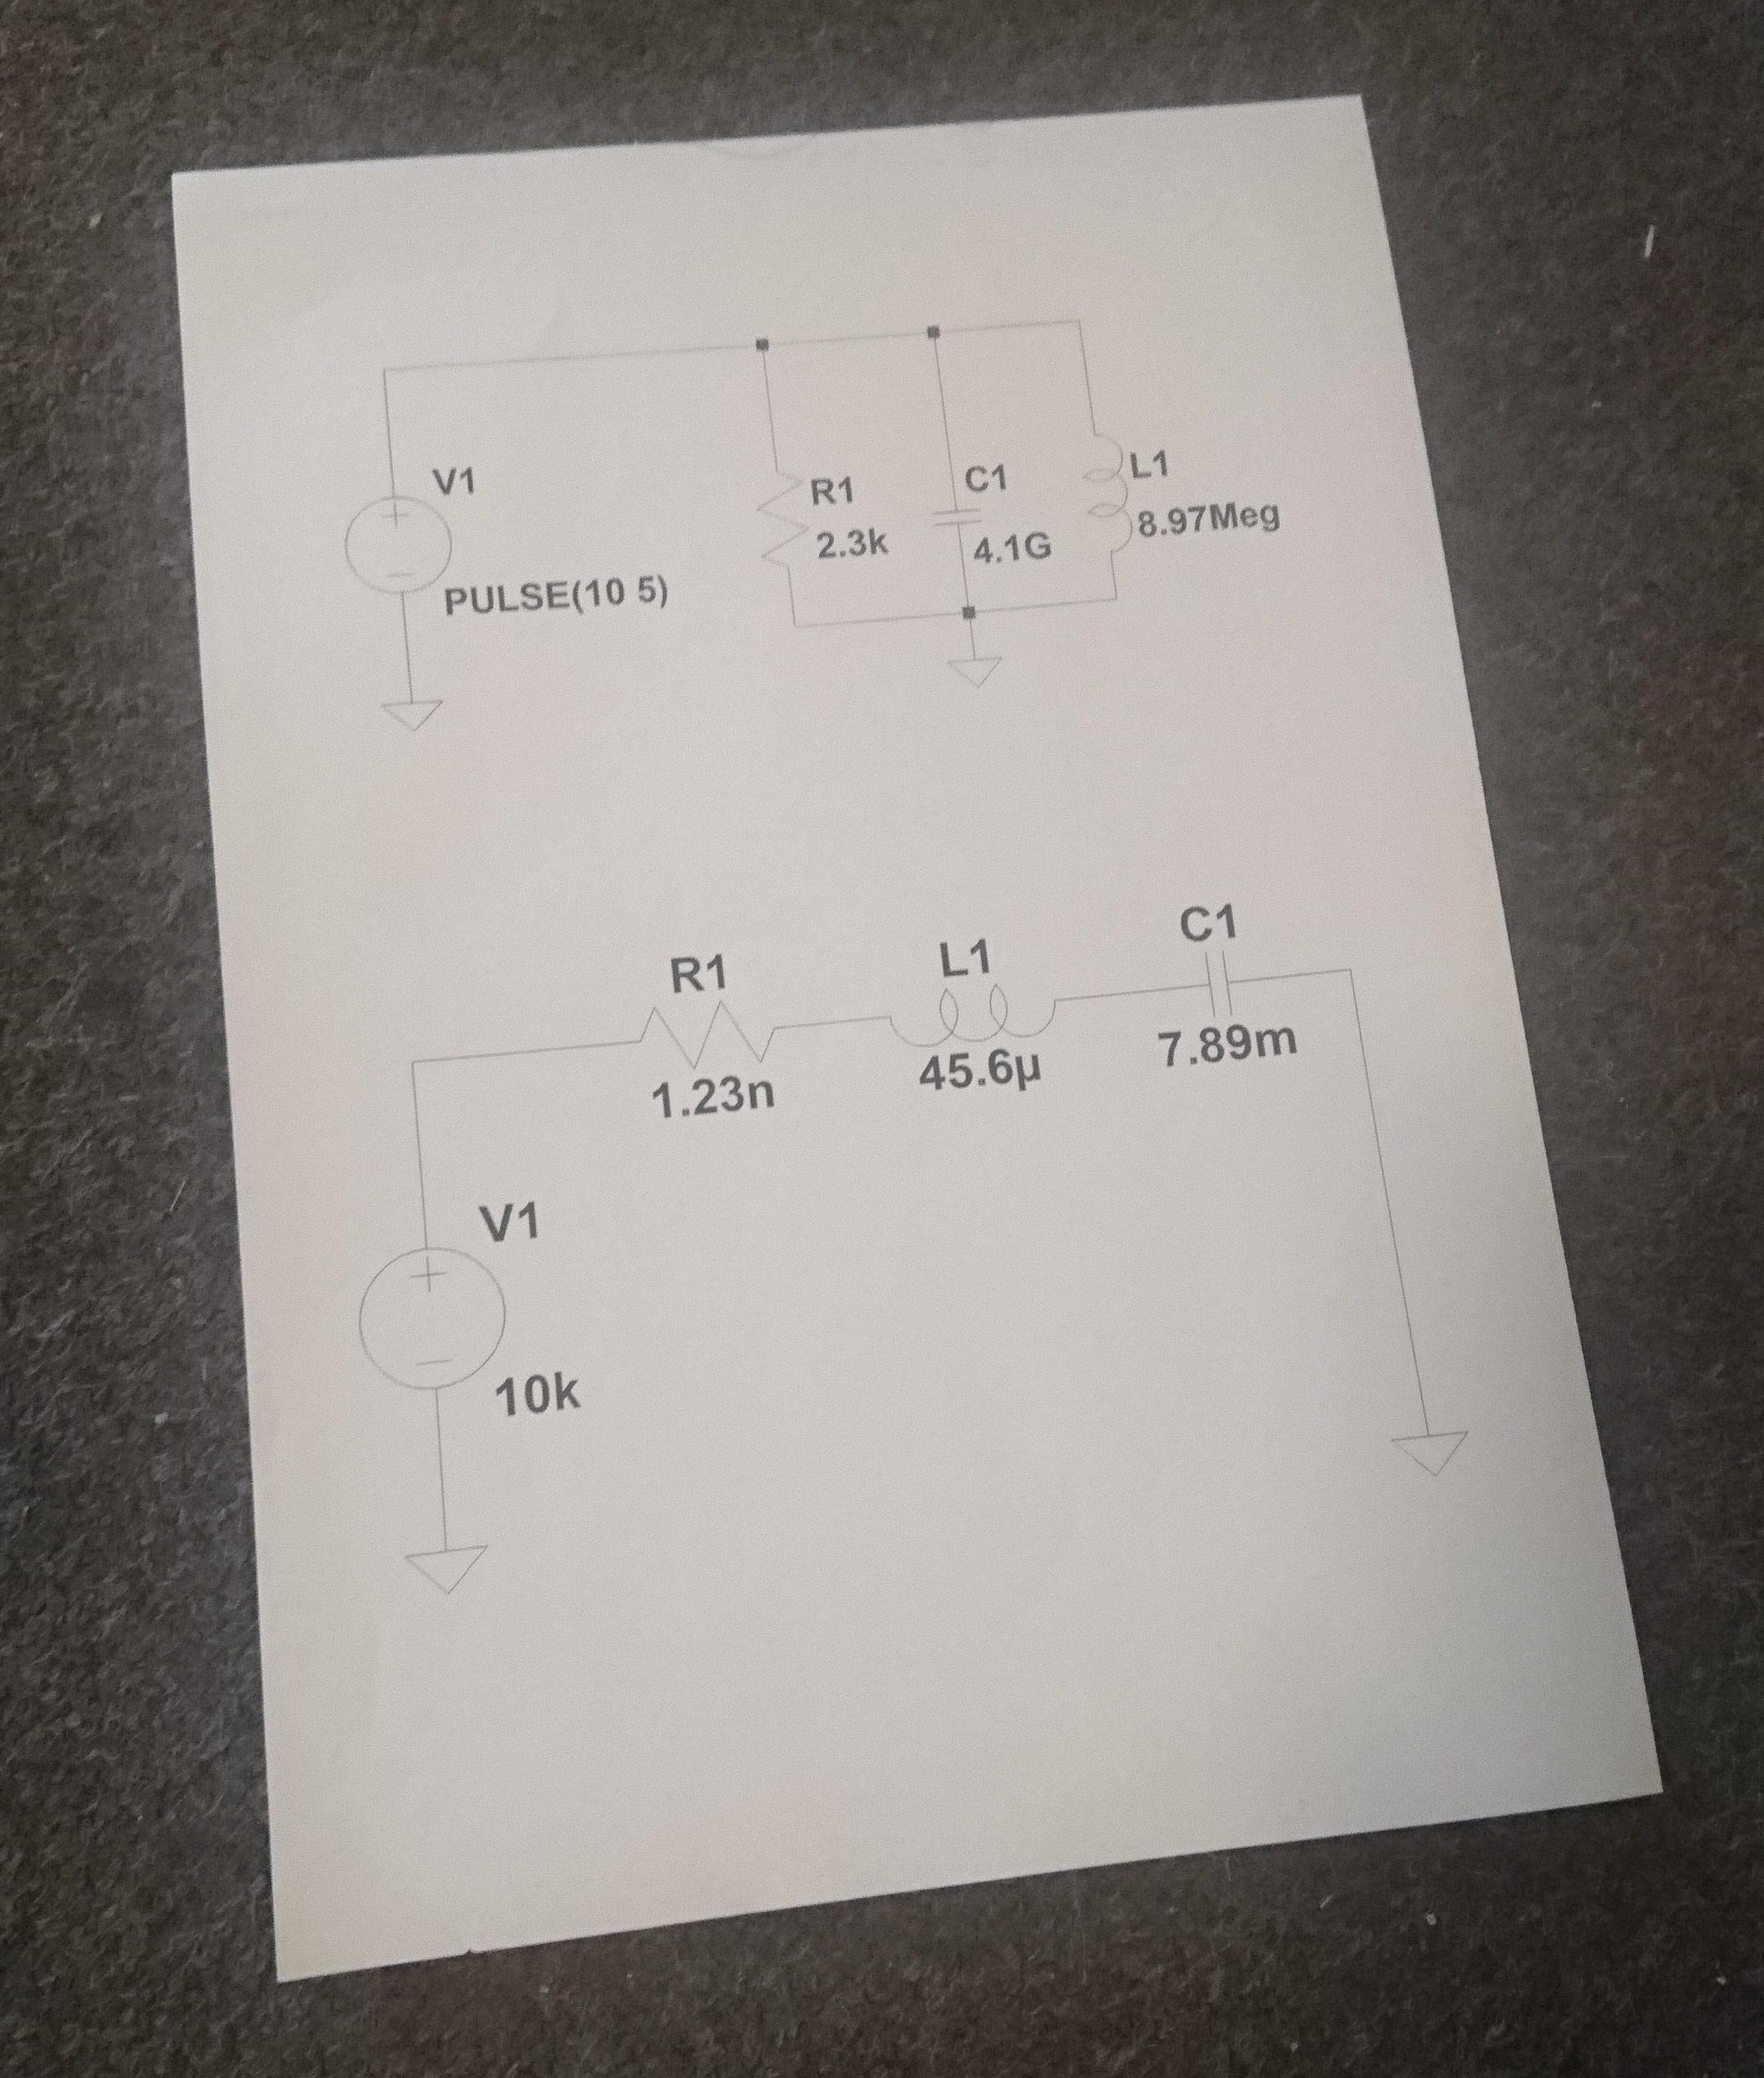
\includegraphics[width = 3.2in]{img/S04.JPG}
\caption{Example photography of a circuit}
\label{fig:c2}
\end{figure}

\par
Initially, the program expects a digital image to be selected by the user. This image can be either a photography of a schematic on a sheet of paper or the image of a digitally created schematic. If the image is a photography, the program will first detect the boundaries of the sheet of paper in order to then rectify the image such that the sheet of paper lies entirely in the image plane. This implies that the entire paper is clearly included in the photography. After rectification, the photo can be treated in the same way digitally created schematic pictures are to be treated.
\par

\begin{figure}[!ht]
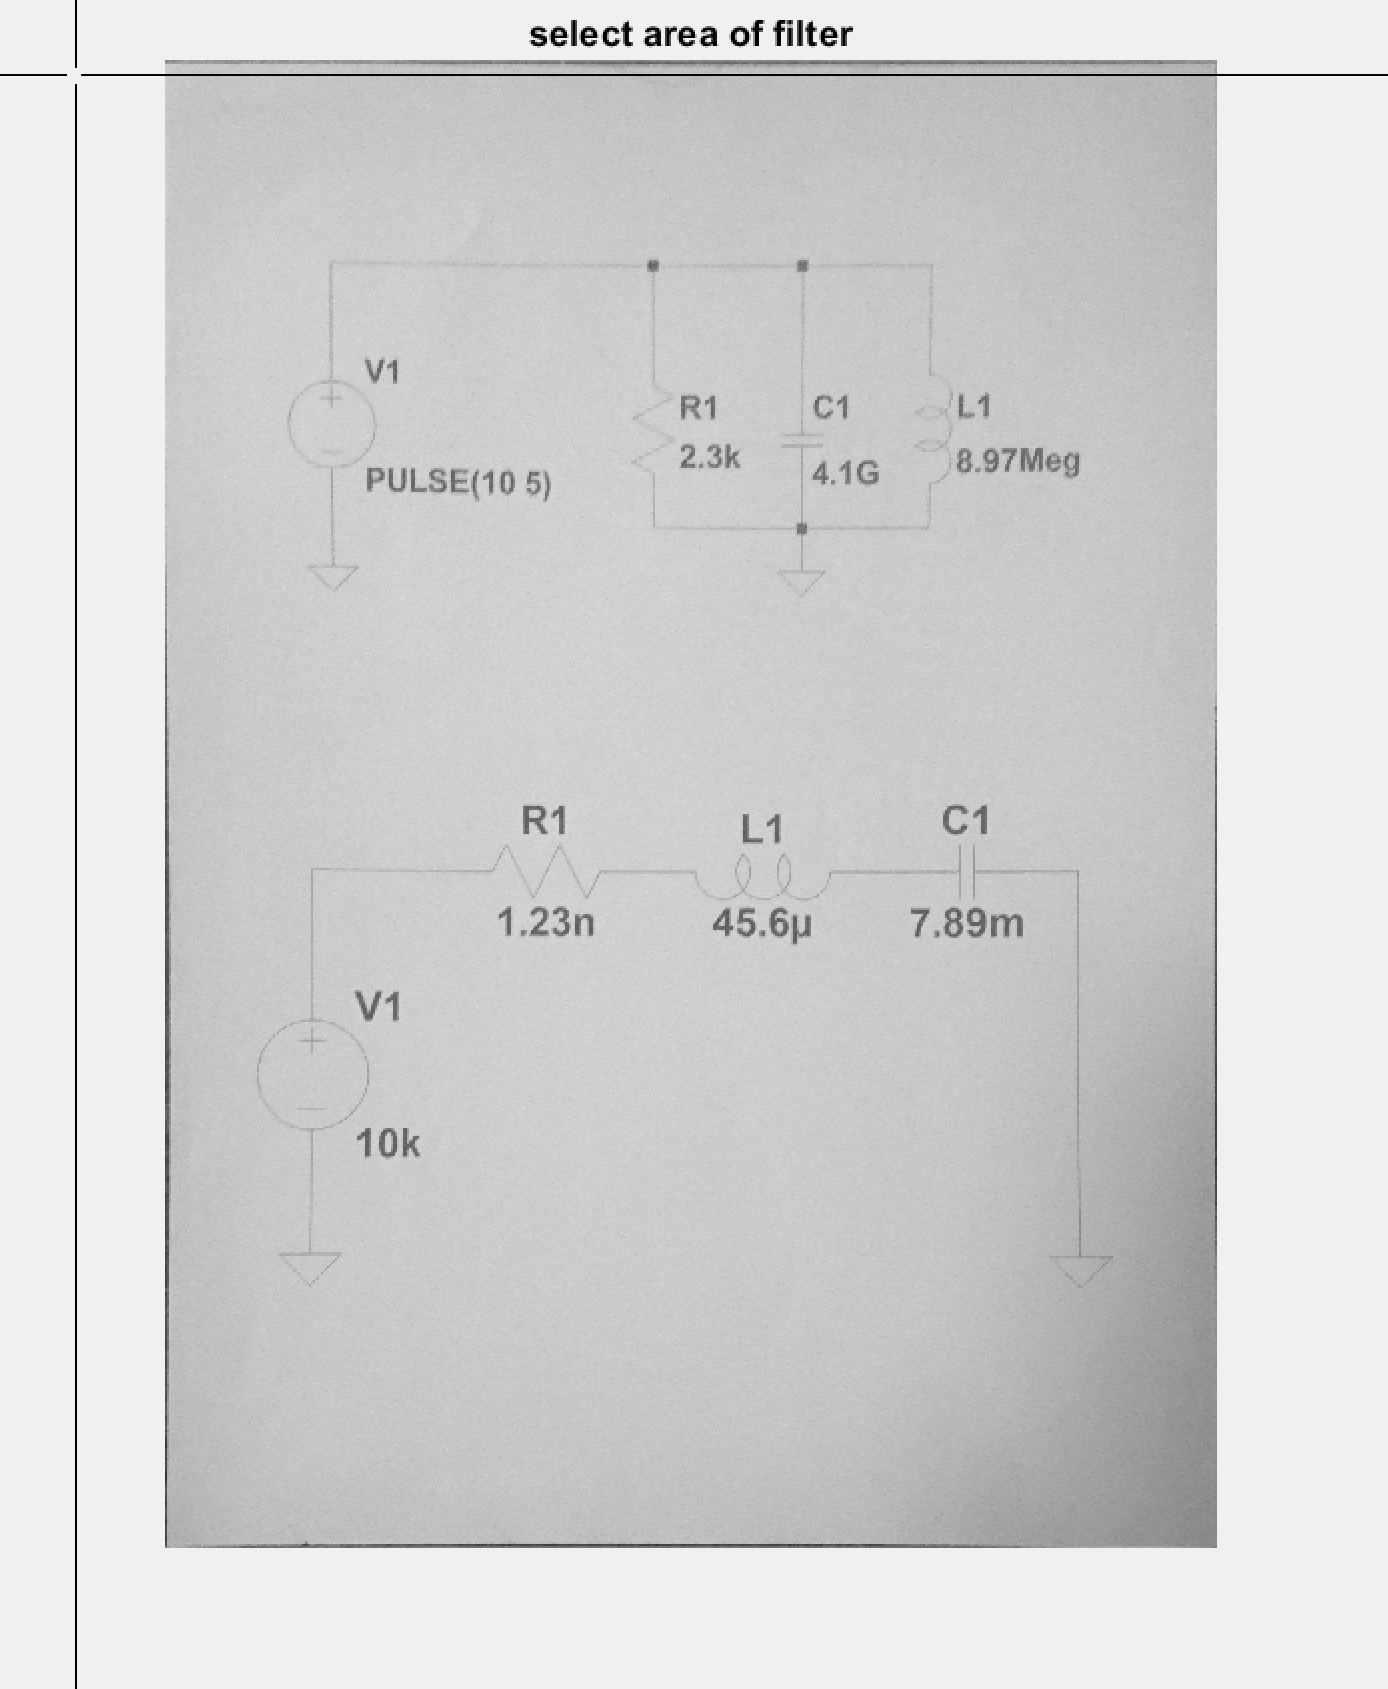
\includegraphics[width = 3.2in]{img/roi.png}
\caption{ROI selection within a rectified photography}
\label{fig:c3}
\end{figure}

\par
The user selects a region of interest (ROI) within the provided (rectified) image; the following analysis will be limited to that specific ROI. The first step of the image analysis algorithm is \textbf{Optical Character Recognition} (OCR), as every electrical element comes with electrical properties textually encoded next to them in the image. Recognized text is stored and deleted from the image. Hereby OCR is running in a loop: After each OCR iteration, the program asks the user to confirm the removal of all text within the selected ROI. If this is not the case, he is asked to manually select new regions of interest so that the OCR routine can obtain and remove the remaining text.
\par
Following up is the \textbf{retrieval of geometric primitives} within the images which will be further explained in subsection \ref{subsec:geom}. Obtained through the binarized and thinned image, these primitives are used to retrieve the scale of the electrical components of the schematic in the image.
\par
Using the knowledge of the components' scale, the \textbf{object detection} is done using a sliding window to retrieve the location and orientation of electrical elements in the image. Following up is the \textbf{detection of wires} based on the image after deletion of the detected elements. See subsections \ref{subsec:obj} and \ref{subsec:wire} for more detailled descriptions.
\par
Finally, after having detected elements and the connections in between, the \textbf{output generation} model uses the objectified results of the image analysis and creates and fills a Simulink model. This model will then be shown and saved for further usage. Refer to section \ref{sec:output} for further imformation.

% MAIN----------------------------------------------------------

\section{Preprocessing}
\label{sec:pre}

Before being able to obtain the electrical circuit elements from the provided image, several steps have to be taken in order to facilitate the information retrieval.

\subsection{Rectification}
\label{subsec:rect}

When dealing with photographies, the depicted schematic may be distorted due to the surface not being aligned to the image plane. This has to be taken care of in order to use the object recognition approach presented in this work. Therefore, asserting that the entire surface and its corner points are included in the image, a rectification step is taken to bring the schematic onto the image plane.
\par

To do this, the image needs to be processed first. After binarizing the image with a predefined threshold, the biggest shape get extracted. This means that we assume the paper to take up the most part of the image. After additional filtering with edge detection and dilating and eroding the result, the remaining holes (mostly text) will be filled so that only a tetragon remains.\\
By taking the boundaries of the image and calculate its mean values we can transform the resulting polar coordinates to Cartesian coordinates.

\begin{figure}[!ht]
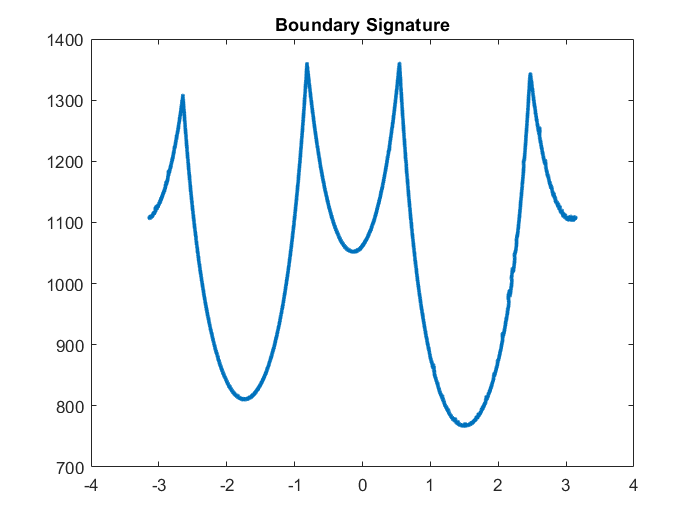
\includegraphics[width = 3.2in]{img/sig.png}
\caption{Boundary signature of a detected paper}
\label{fig:sig}
\end{figure}

Figure \ref{fig:sig} shows the result of that transformation. Taking the value of the peaks with the highest prominence the location of the edges can be found. With the resulting points, the corresponding points need to be generated. This is done by taking the mean value of the point pairs (which are defined by the pair that is the closest together). After that the aspect ratio will be corrected to be identical to that of a \textit{A4} paper. After a simple warping of the image the edges get detected again to verify the result and the image gets cropped according to the result.

\par

\begin{figure}[!ht]
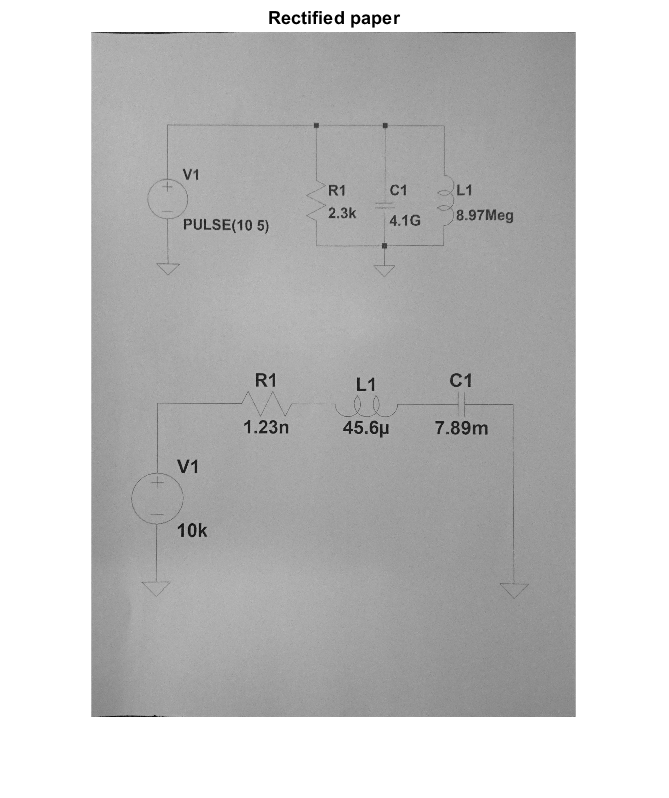
\includegraphics[width = 3.2in]{img/rect.png}
\caption{Post-rectification of image in figure \ref{fig:c2}}
\label{fig:c5}
\end{figure}

\subsection{Optical Character Recognition}
\label{subsec:ocr}

In depictions of non-distorted or rectified schematics, MATLAB's OCR functionality can be used to retrieve text and its position within the image. After retrieval, the corresponding text regions in the image are erased, simplifying the following recognition of electrical elements and connections.
\par

\begin{figure}[!ht]
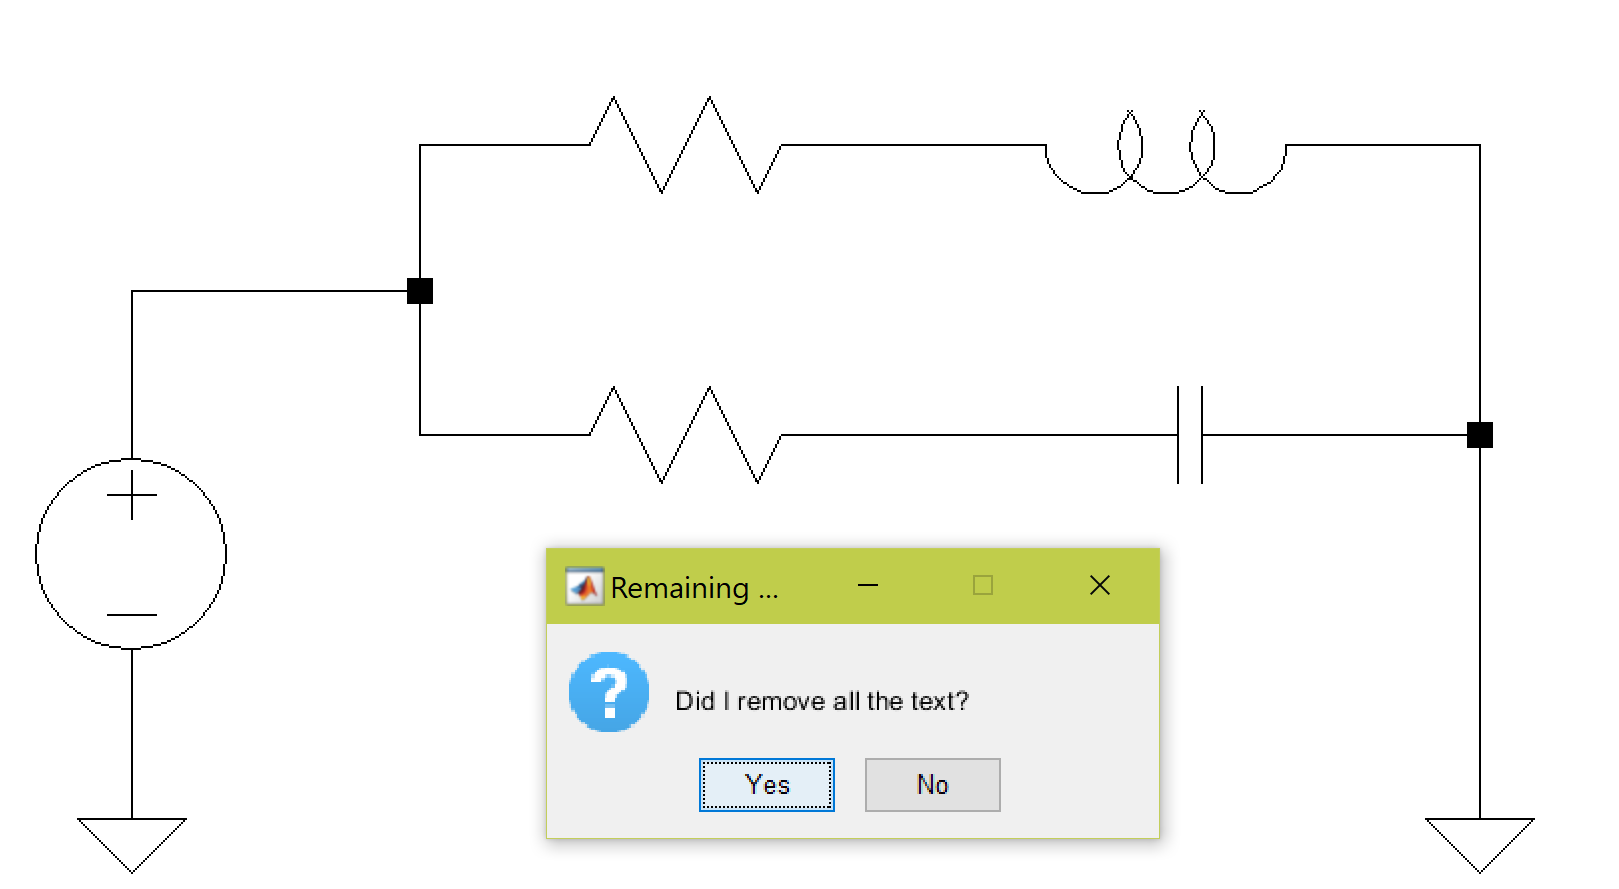
\includegraphics[width = 3.2in]{img/ocr.png}
\caption{Successful OCR result}
\label{fig:ocr}
\end{figure}
\par

For the OCR function a specific language was trained using the \textit{MATLAB} training function. This gives more precise results, as only letters contained in \textit{RLC}-filter circuits are allowed (and component values between $p$ and $G$). All values that have been found to be above a predefined confidence (depending on photo or screenshot) will be extracted and the text will be erased from the image. If not all text was found successfully (if the text is too close to a component), the user can define the region where the rest of the text lies (with the confidence lowered). If the image comes from a photo, some adaptive and noise filtering will be done before the OCR and some line thickening afterwards since the image will have more grey scale values compared to the screenshot. Figure \ref{fig:ocr} shows the successful result of the algorithm.

\subsection{Binarization, Morphology}
\label{subsec:morph}

After all text has been recognized and erased from the image, a binarized and thinned-out version of the image is prepared to further facilitate the following retrieval of lines, circles, corners and element template matchings. Both operations are done using pre-defined functions within MATLAB.
\par

% ---------------------------

\section{Image Analysis}
\label{sec:analysis}

The goal of the functions within the image analysis package is to retrieve all objects from the pre-processed image. This includes the electrical components themselves as well as the wires connecting them. The approach used for the detection of the electrical components is a sliding-window approach, implying that a robust estimation of the scale electrical components is essential in order to find the objects quickly. This in turn calls for the usage of geometric primitives in order to determine that scale.

\subsection{Geometric primitive retrieval}
\label{subsec:geom}

\begin{figure}[!ht]
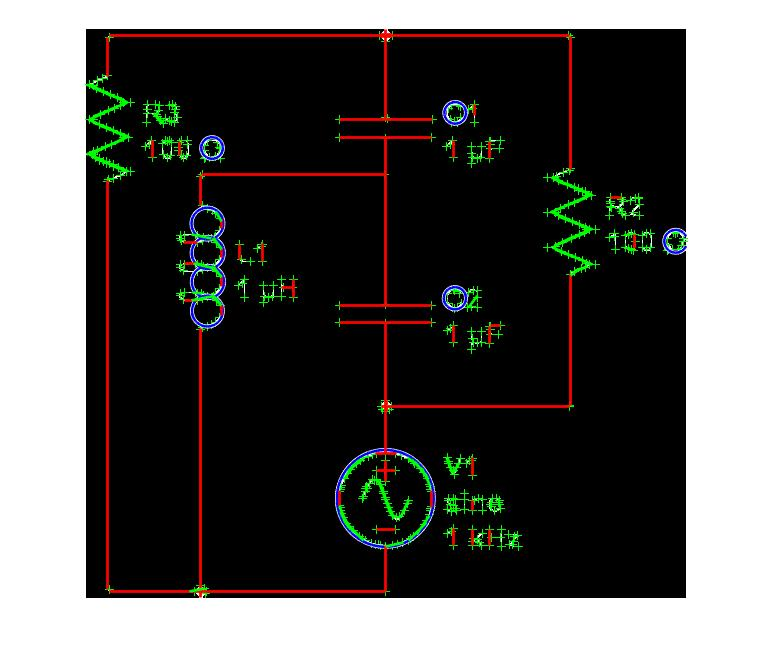
\includegraphics[width = 3.2in]{img/geomprim.jpg}
\caption{Retrieved geometric primitives: circles in blue, lines parallel to the axes in red, skewed lines in green and corners as green crosses.}
\label{fig:c8}
\end{figure}
\par

For lines, a parametrized hough transformation is used. The results are rearranged into a data structure including length and angle of all lines, using the given start- and endpoints of the lines.
\par
For circles and corners, which are unused in the current version of the program, predefined MATLAB functionality is used to detect the harris features of the image and the centers and radii of circles are found using a circular hough transform.
\par
In order to retrieve the scale of the elements, skewed lines are used because in rectified schematics conforming to LTSpice, they are used in resistors only. They can be used to retrieve their dimensions, when assuming that every schematic has at least one resistor and every resistor is conforming to the LTSpice regulations. Then, the greater one of the coordinate differences of full-length lines (of which one is highlighted in Image \ref{fig:c9}) along the axes corresponds to the shorter side of the resistor whereas four times the coordinate difference along the other axis corresponds to the longer side of the resistor.
\par

\begin{figure}[!ht]
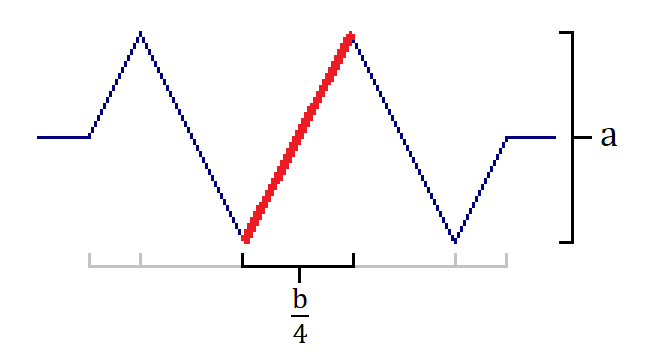
\includegraphics[width = 3.2in]{img/resdim.png}
\caption{Resistor template with highlighted full-length line and resistor dimension explanations}
\label{fig:c9}
\end{figure}

\par
Using this heuristic, the size of a resistor can be estimated within tolerance of a few pixels. Furthermore, including the stretched half-length lines which lie at the end of resistors, the algorithm becomes more robust.

\subsection{Object Detection}
\label{subsec:obj}

The general approach used for object detection is a sliding-window approach. The structure of object detection goes as follows: 
\begin{itemize}
	\item Specific pre-processing for object detection
	\item Sliding window: Generation of an error-image (difference from template to reference)
	\item Get position of minimum error/maximum correlation
	\item Ranking and selecting candidates
	\item Return found elements
\end{itemize}

\subsubsection*{Preprocessing for Object Detection}

Before the sliding window can be applied, the image needs to undergo specific preprocessing, which is an integral part of object detection. The template (i.e. a resistor) and the reference image (i.e. the circuit) are first binarized, scaled down for performance and then dilated. The dilating factor is an essential parameter and influences how tolerant the algorithm is of dissimilarities between the template image and actual representations of the template in the reference image. Increasing the dilation factor increases the change to find high-correlation areas but also decreases accuracy and precision. In figure \ref{fig:detPP1} and figure \ref{fig:detPP2} we can see a template and a reference image being (heavily) dilated. A scaling factor between 0.1 and 0.4 proofs to be both relative fast and still returns good results.
\par

\begin{figure}[!ht]
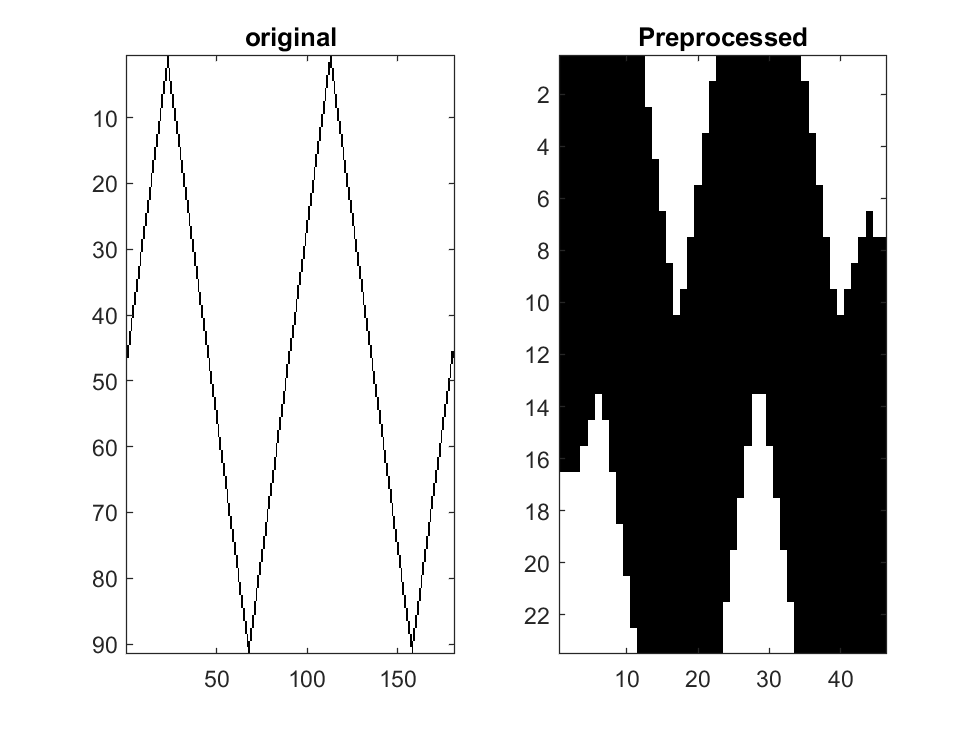
\includegraphics[width = 3.2in]{img/detPP1.png}
\caption{Dilated template}
\label{fig:detPP1}
\end{figure}
\par

\begin{figure}[!ht]
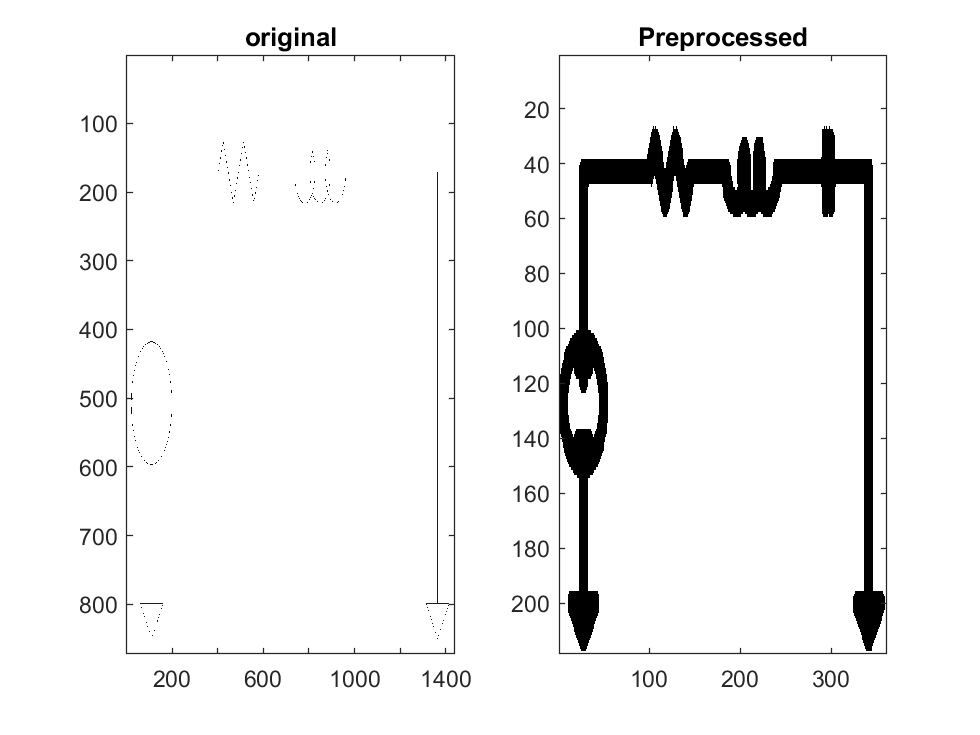
\includegraphics[width = 3.2in]{img/detPP2.png}
\caption{Dilated reference image}
\label{fig:detPP2}
\end{figure}

\subsubsection*{Sliding window and error-image}

The preprocessed template is now sliding over the reference image, while a normalized mean-squared error (or difference value) is calculated at each position. The error values form the error image. Figure \ref{fig:detSW1} and\ref{fig:detSW2} each show a dilated reference image on the left and the corresponding error visualization on the right. Hereby, figure \ref{fig:detSW1} shows much lower dilation values than figure \ref{fig:detSW2}. Observing the error patterns, it is clear that the highly dilated image yields better results, but also more maxima where none should be.
\par

\begin{figure}[!ht]
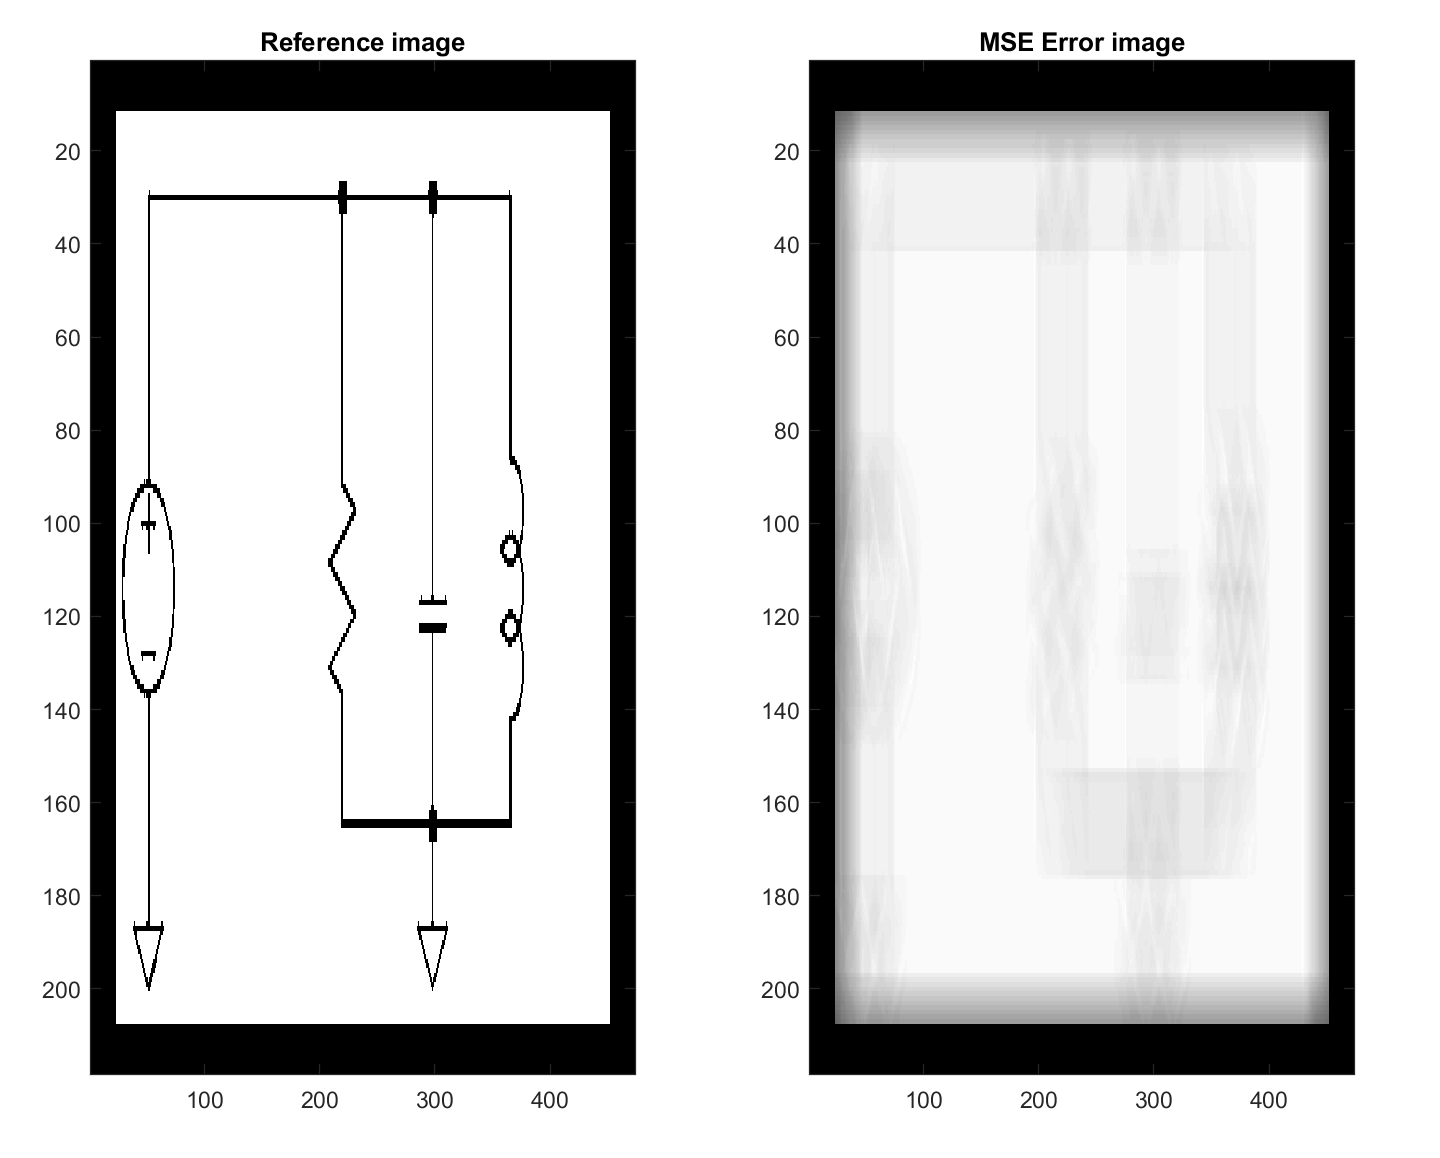
\includegraphics[width = 3.2in]{img/detSW1.png}
\caption{Slightly dilated reference image and resulting error image}
\label{fig:detSW1}
\end{figure}
\par

\begin{figure}[!ht]
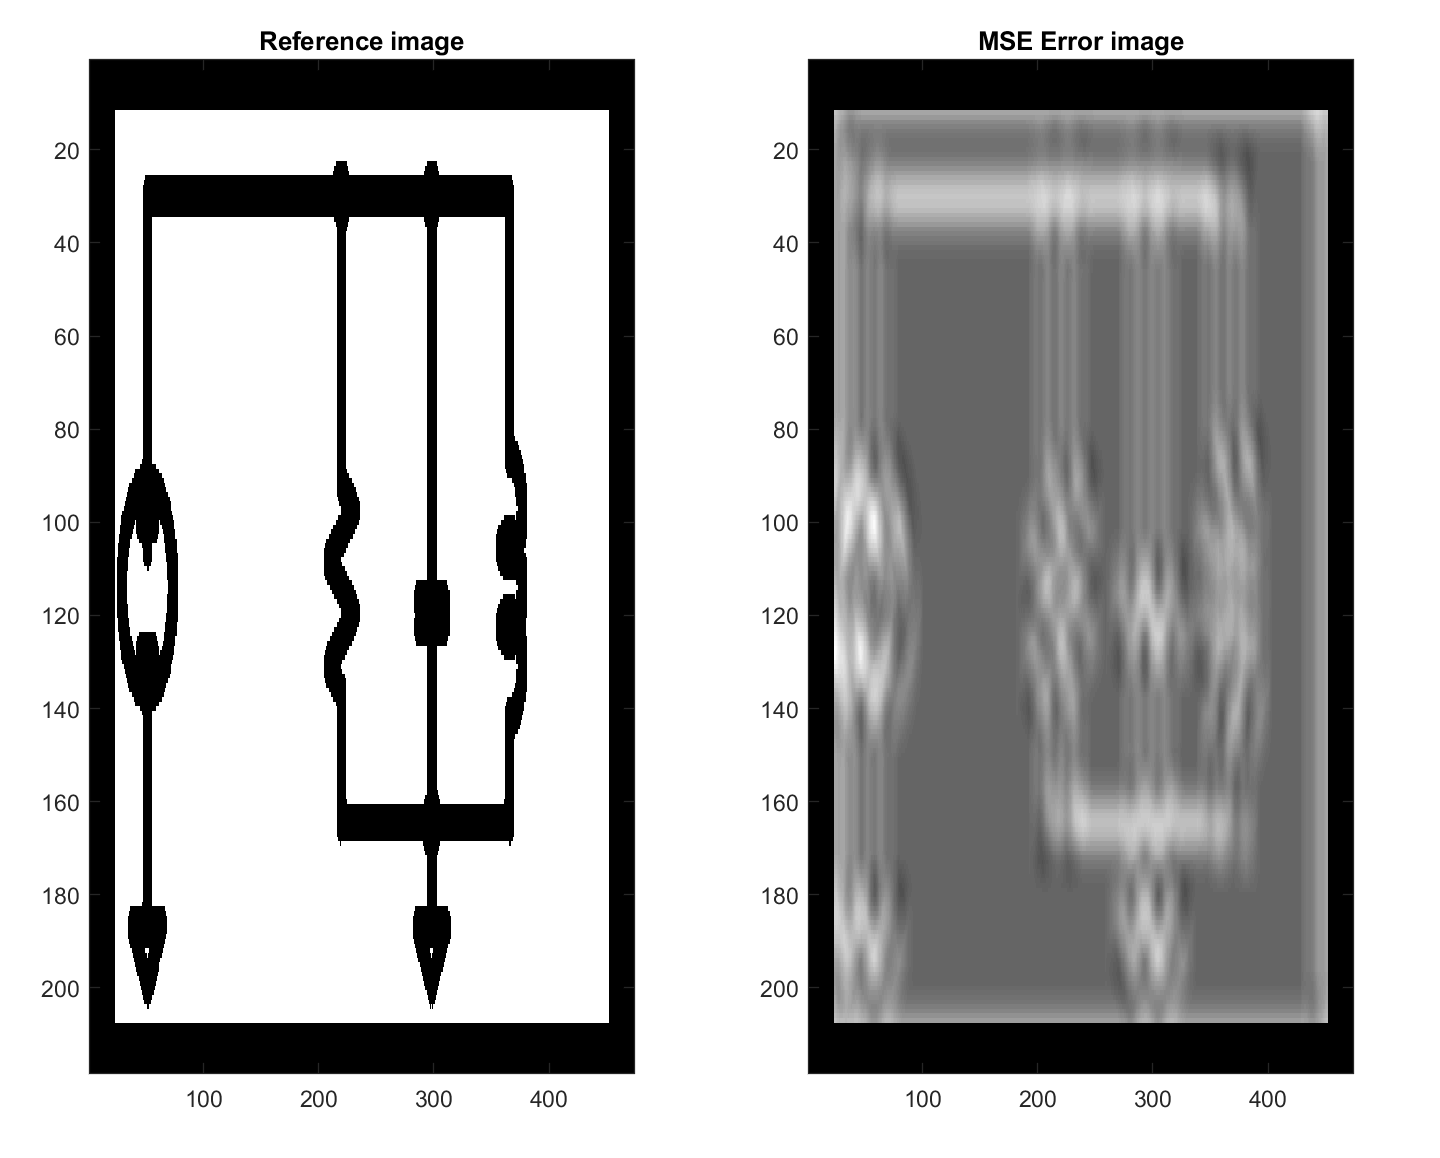
\includegraphics[width = 3.2in]{img/detSW2.png}
\caption{Heavily dilated reference image and resulting error image}
\label{fig:detSW2}
\end{figure}

\subsubsection*{Get Maximum Correlation}

Using the error image (or inverted: the correlation image), the algorithm tries to find significant maxima in the image. Noise and similarities between objects (e.g. grounds and resistors, or capacitors and wires) make the search for maxima difficult. The algorithm first supresses all values below a certain dynamic threshold and then binarizes again, using another dynamic threshold. Occasionally, the final binarization fails to produce good results and higher dilation values must be used. 
\par
Figure \ref{fig:detMX1} to \ref{fig:detMX3} show the different attempts to identify a capacitor, which is particularly hard to detect with certainty due to its very simple geometric shape. In figure \ref{fig:detMX1}, the target maximum is not significant enough and its value is too close to the rest of the error-image. The final binarization results in an all positive image. In figure \ref{fig:detMX2}, other areas have significant - although faulty - maxima aswell, resulting in a faulty final binarization. Figure \ref{fig:detMX3} shows a successful suppression of minima and a successful binarization, with an isolated, significant dot as result. 
\par
The algorithm detects those isolated dots and decides whether it has found an object at concerned position, whether it needs to use different parameters or whether there is no element of this kind to be found.
\par

\begin{figure}[!ht]
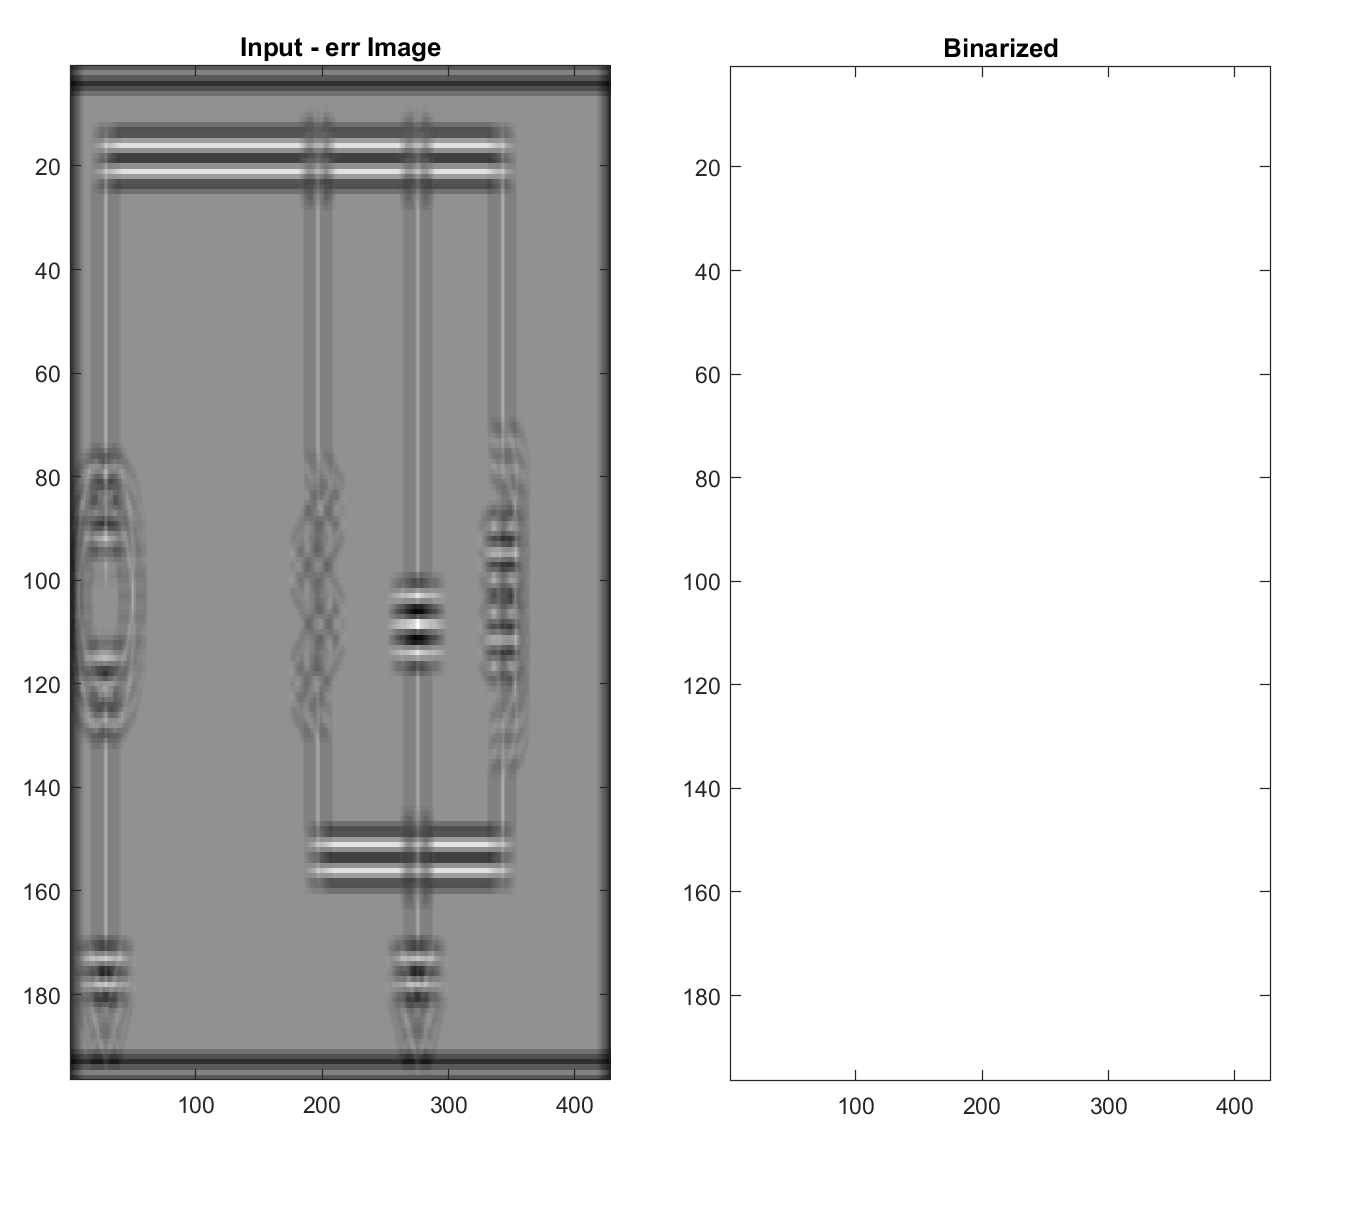
\includegraphics[width = 3.2in]{img/detMX1.png}
\caption{Faulty binarization - main maximum too insignificant}
\label{fig:detMX1}
\end{figure}
\par

\begin{figure}[!ht]
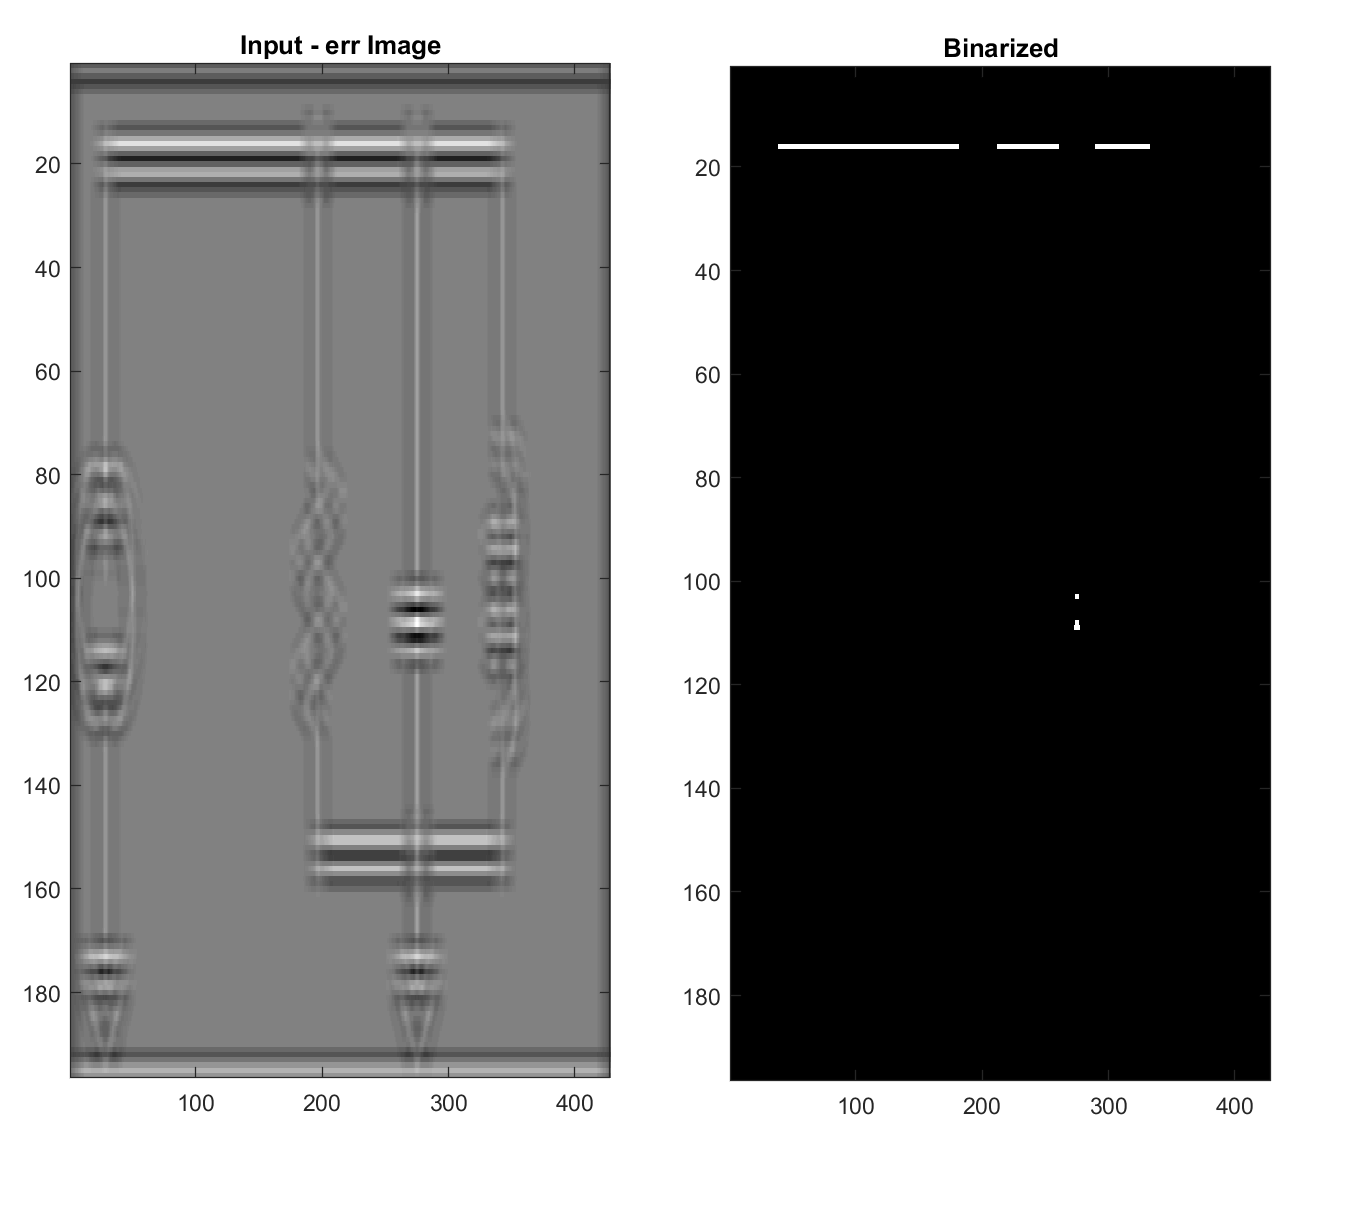
\includegraphics[width = 3.2in]{img/detMX2.png}
\caption{Faulty binarization – false maxima detected}
\label{fig:detMX2}
\end{figure}
\par

\begin{figure}[!ht]
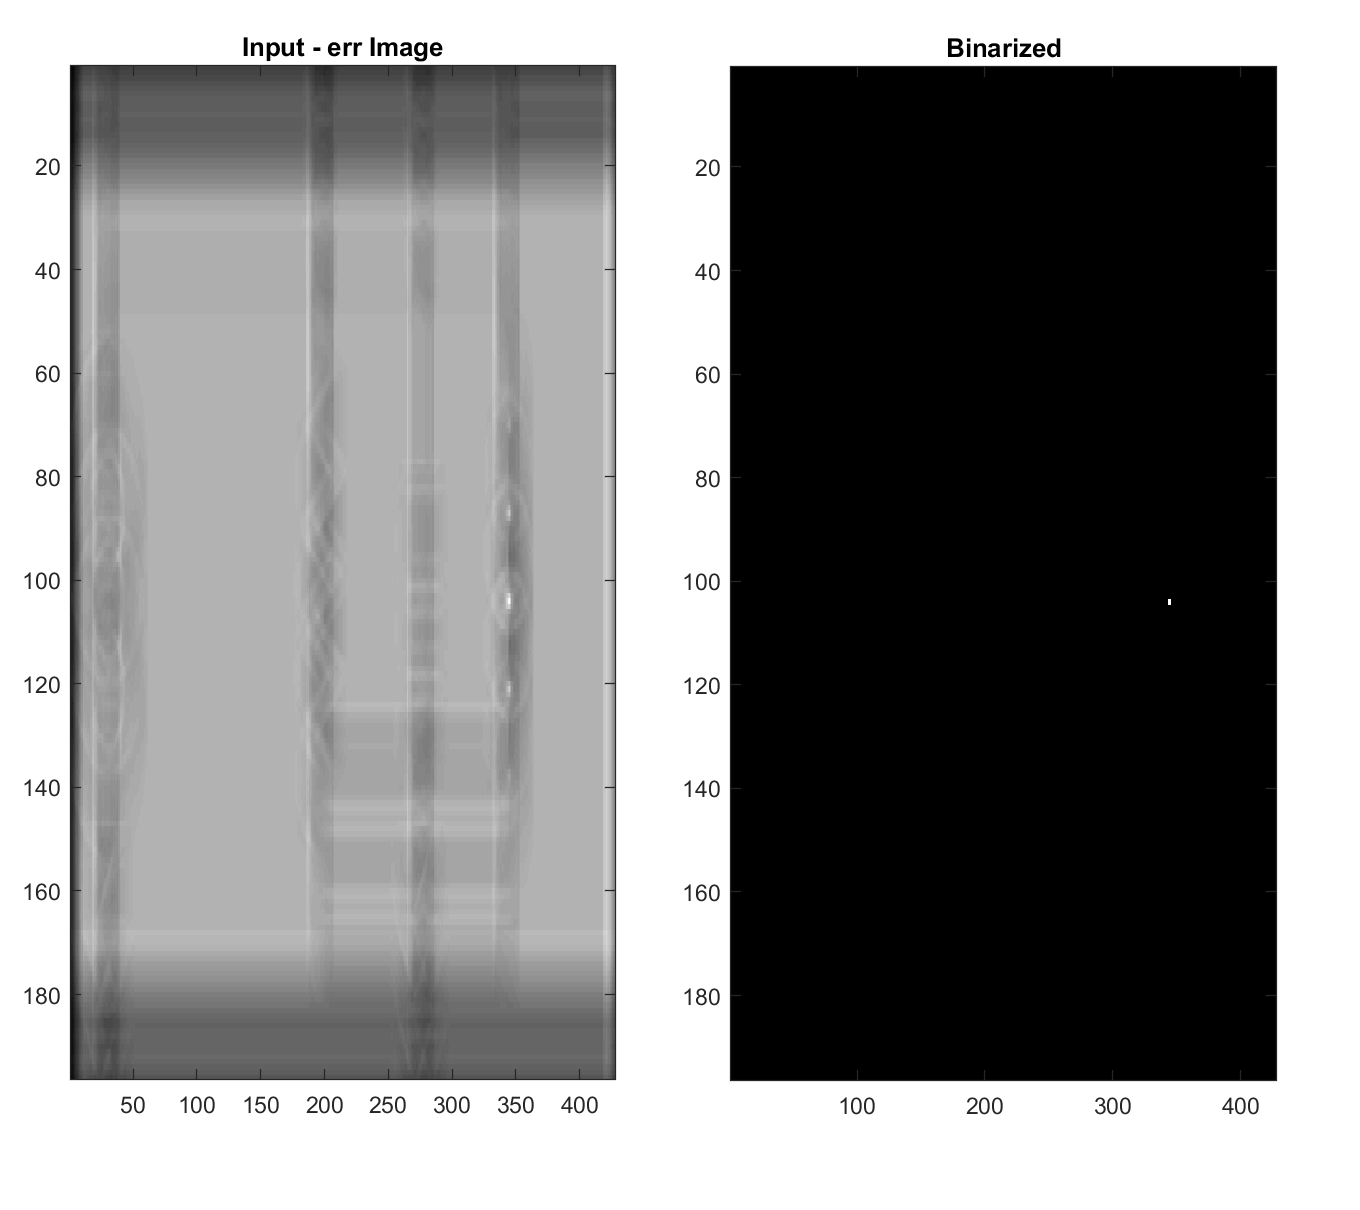
\includegraphics[width = 3.2in]{img/detMX3.png}
\caption{Successful binarization}
\label{fig:detMX3}
\end{figure}

\subsubsection*{Ranking and Selecting Candidates}

As mentioned before, the algorithm is prone to confuse different elements with each other, provided they share geometric similarities. When dilating template and reference image, this confusion gets worse as the tolerance for non-perfect matches increases. Frequently, multiple elements are detected (with varying tolerance) in the same area in the reference image. To counteract this, the algorithm assigns a score to each found element relating to its certainty. After the algorithm searched for all elements, it checks whether the found elements are out of bounds (the edges of the reference image are prone to faulty maxima) and compares their store against each other. 
\par
Figure \ref{fig:detRS1} shows all found candidates for this particular example. Attached to each found element is a confidence score, with lower scores being better. When two or more elements occupy the same area, the element with the lower score gets priority and the others are deleted. The result of this selection process can be seen in figure \ref{fig:detRS2}.

\begin{figure}[!ht]
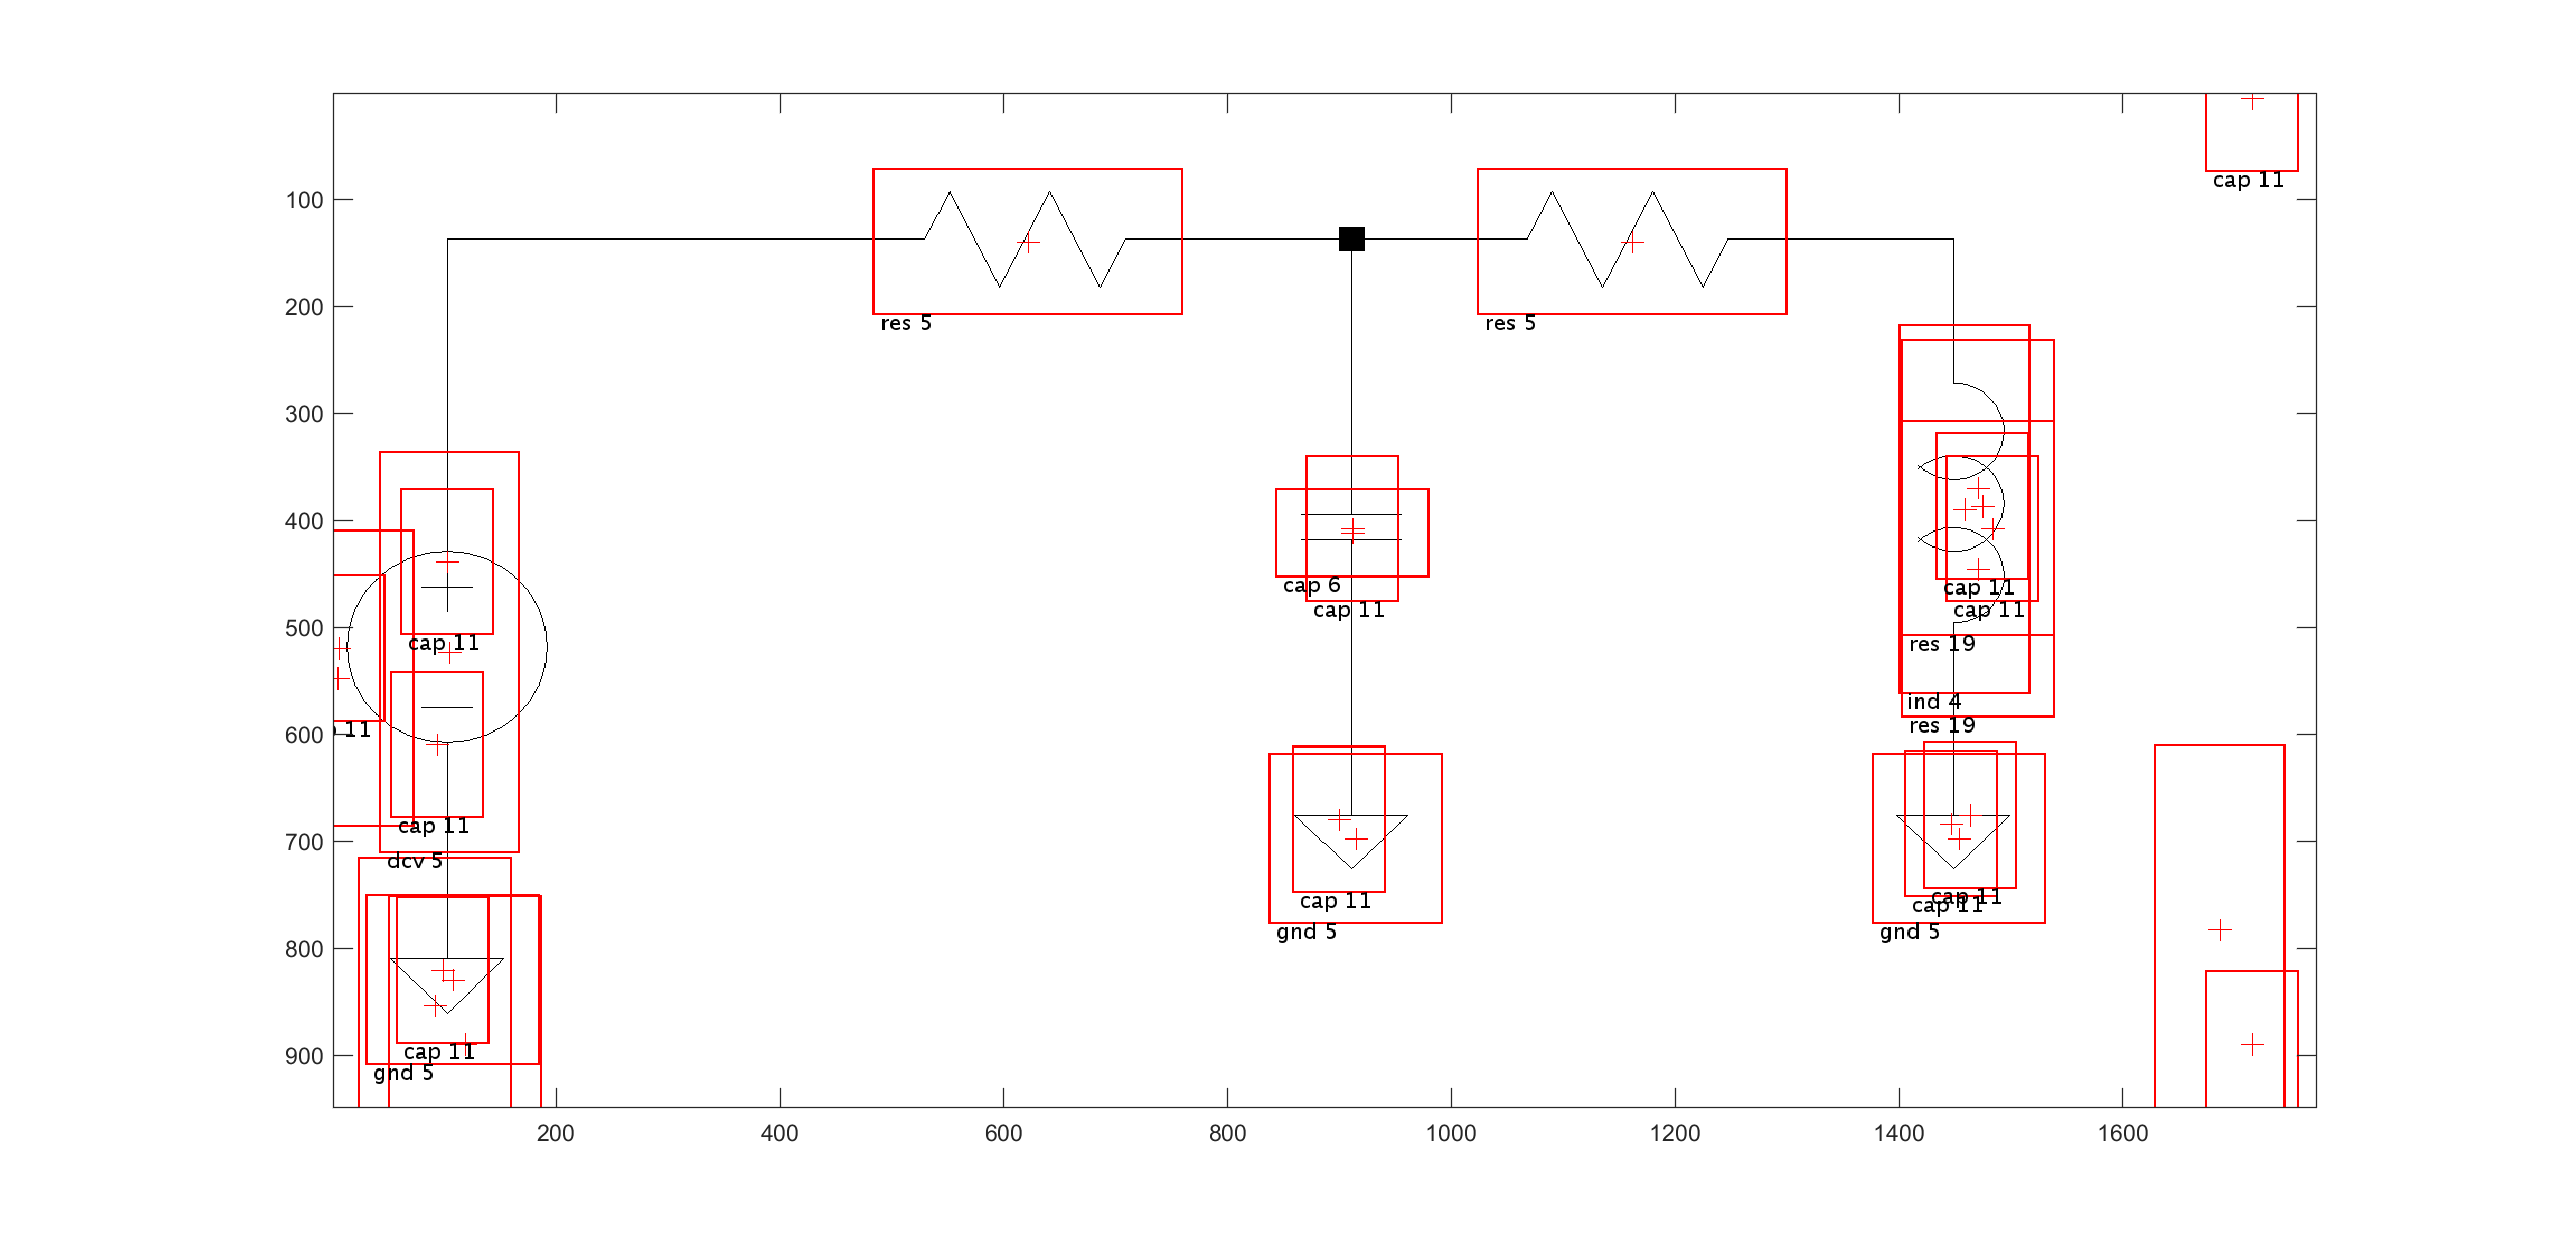
\includegraphics[width = 3.2in]{img/detRS1.png}
\caption{All candidate elements with scores}
\label{fig:detRS1}
\end{figure}
\par

\begin{figure}[!ht]
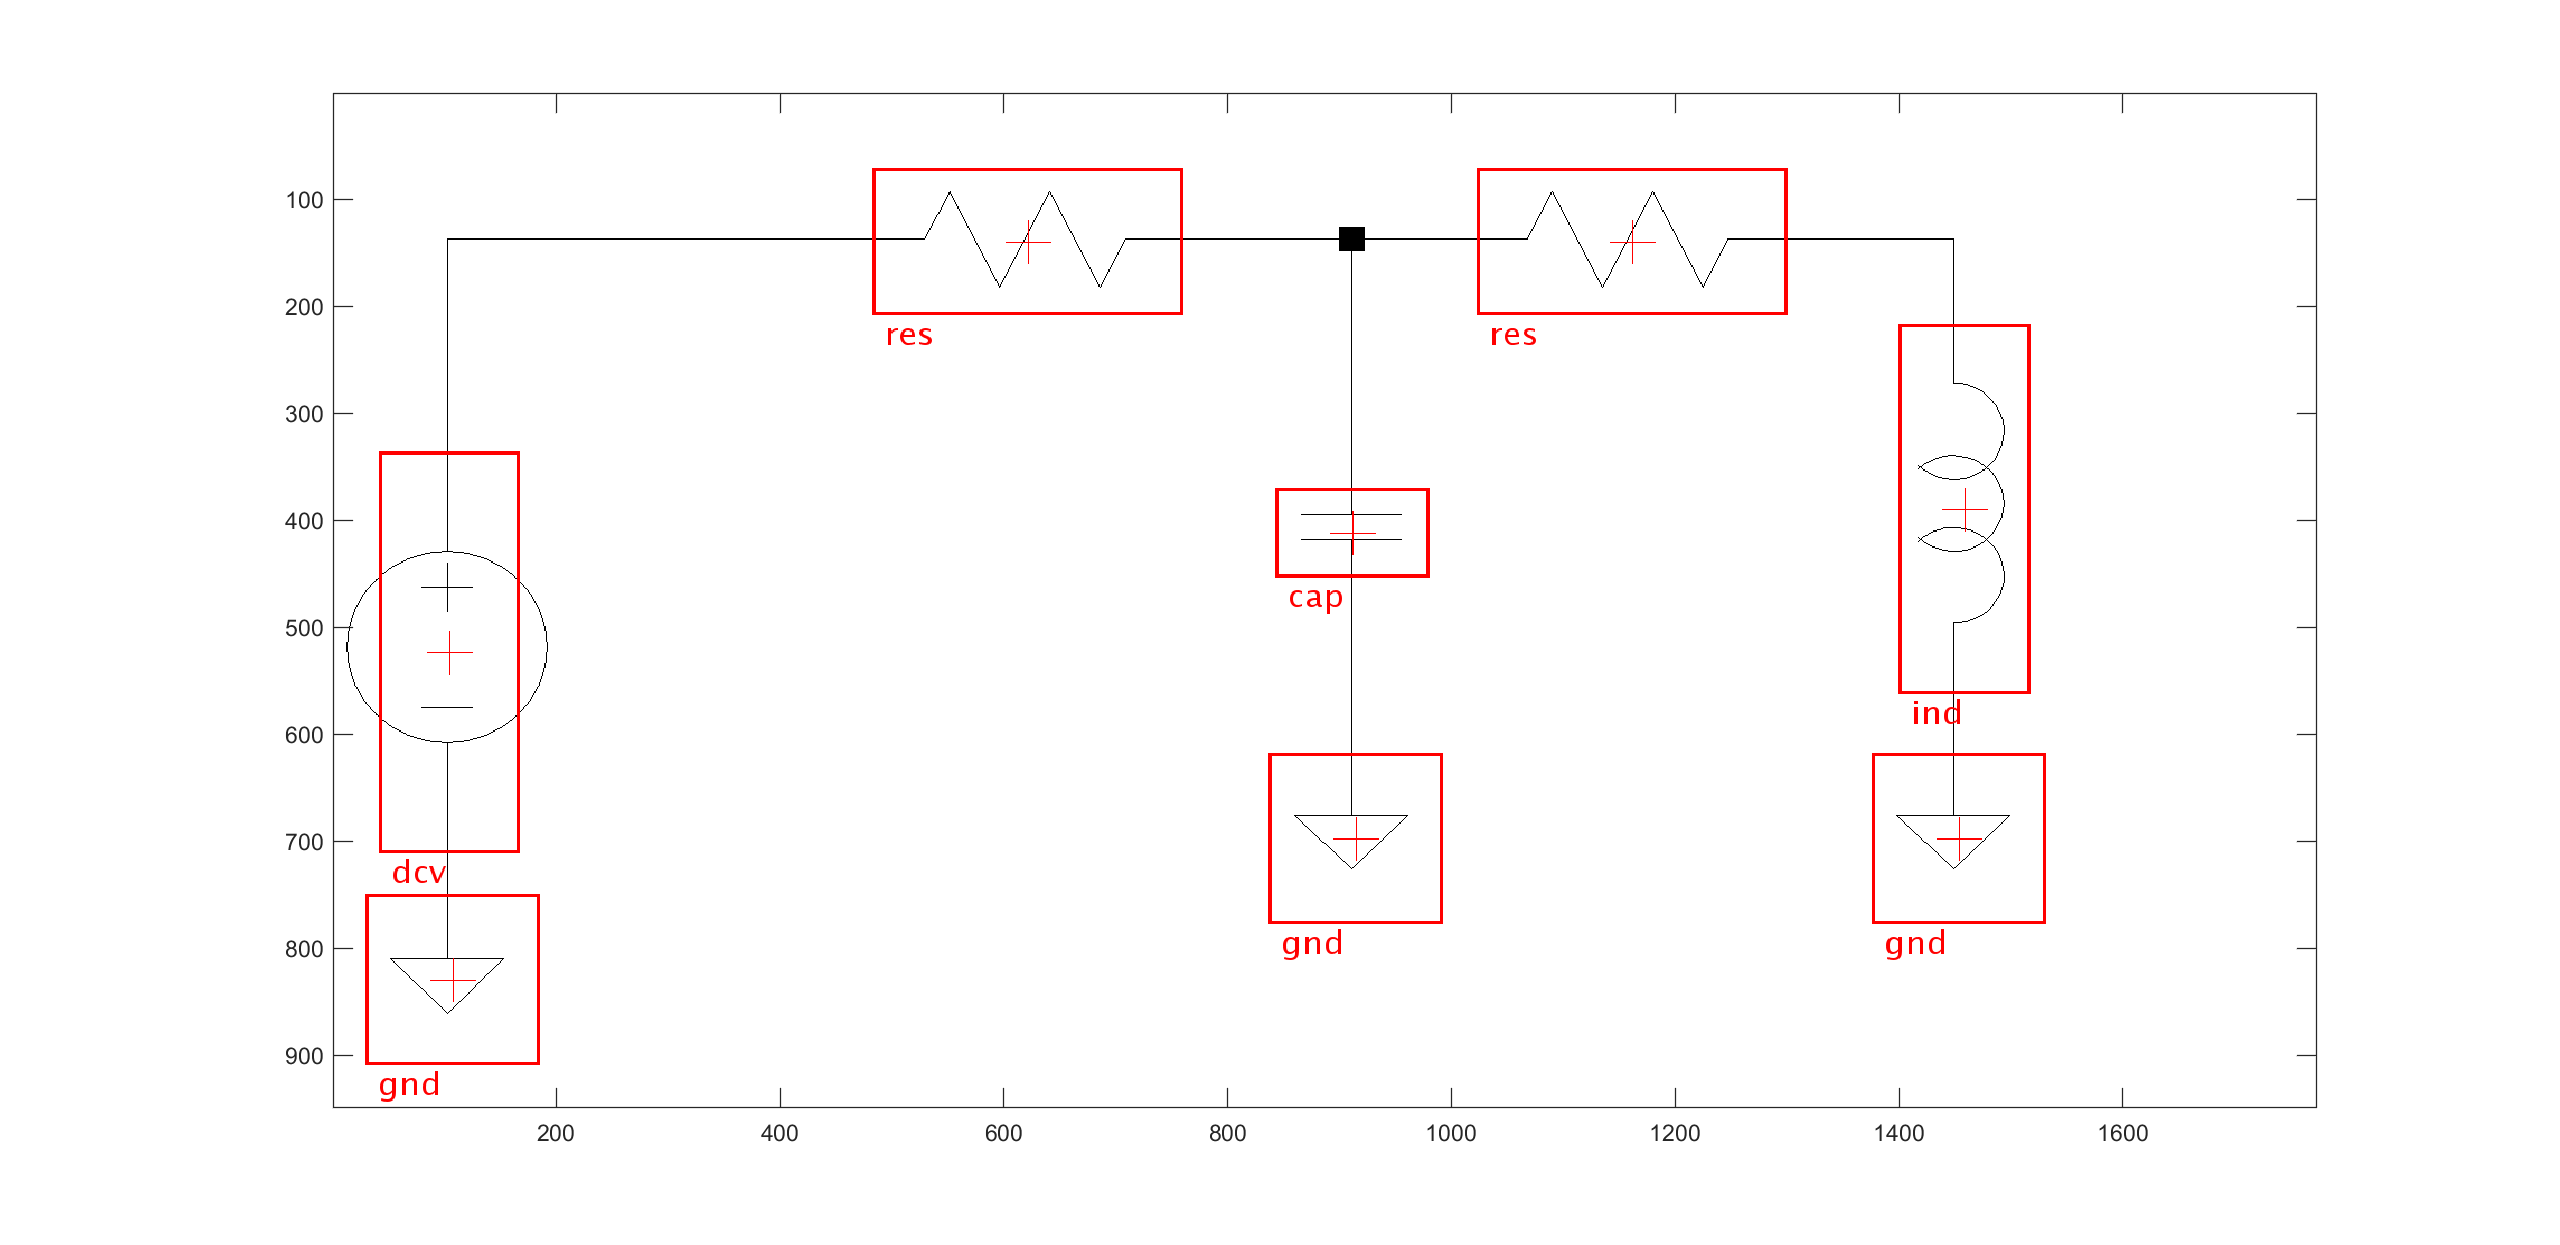
\includegraphics[width = 3.2in]{img/detRS2.png}
\caption{Selected candidates (final result)}
\label{fig:detRS2}
\end{figure}

\subsubsection*{Return Found Elements}

The found and selected elements are stored and returned to the main image analysis function for further processing. In the image, the areas of the found elements are erased to enable the following wire detection.

\subsection{Wire Detection}
\label{subsec:wire}

After having detected the electrical elements and after having erased them from the image, cables and connections are the only entities left in the image. Therefore, a second hough transformation application retrieves the endpoints of the connections between elements.
\par

\begin{figure}[!ht]
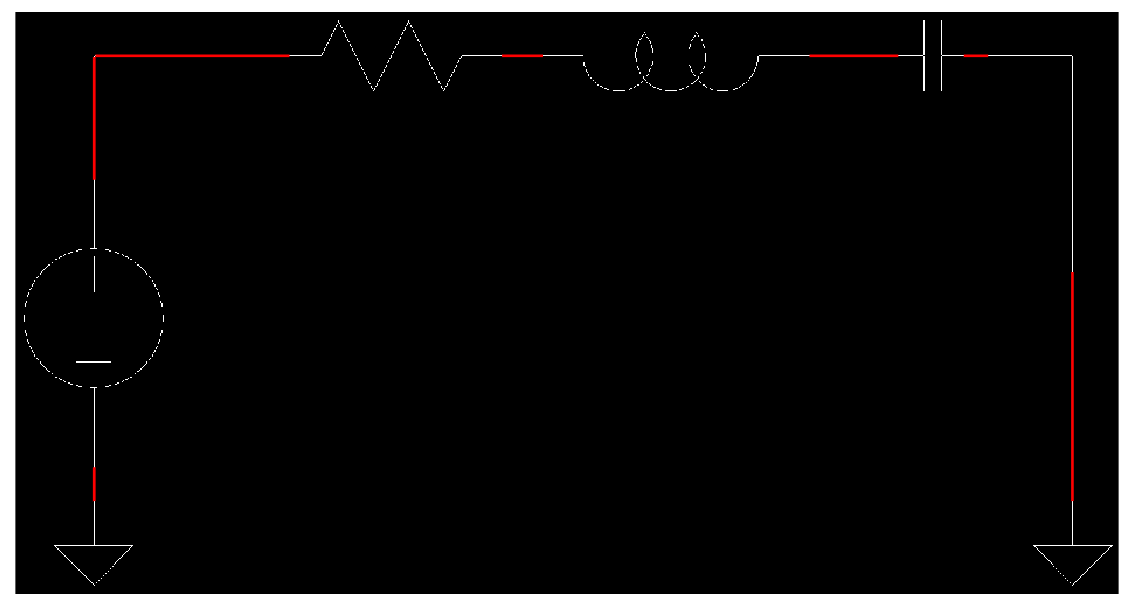
\includegraphics[width = 3.2in]{img/connections_after.png}
\caption{Circuit from figure \ref{fig:detPP2} with recognized cables in red.}
\label{fig:c10}
\end{figure}

\par
After the wire detection, all detection results are passed onto the output generation module.

% ---------------------------

\section{Output Generation}
\label{sec:output}

In this module, the results of the image analysis routines are reframed and sent to SIMULINK in order to build an electrical circuit model. After its creation, the user can interact with the model which is also saved to enable further usage.

\subsection{SIMSCAPE Electrical Model}
\label{sec:sims}

TODO Chris describe Model
\par

\begin{figure}[!ht]
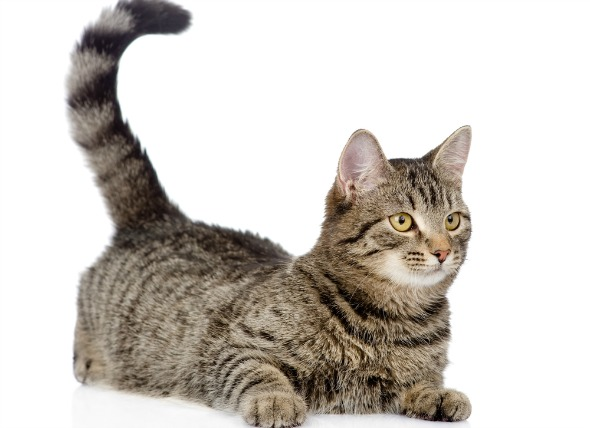
\includegraphics[width = 3.2in]{img/cat.jpg}
\caption{some model pic}
\label{fig:c11}
\end{figure}

\subsection{Component Generation and Assembly}
\label{sec:generation}

TODO Chris describe the reshaping of our data so that you can use the SIMSCAPE Api
\par

\begin{figure}[!ht]
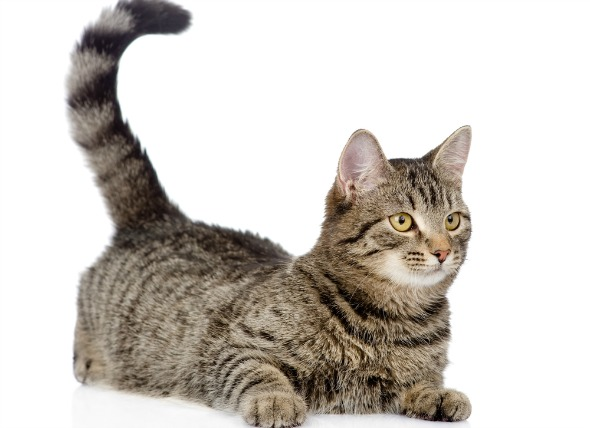
\includegraphics[width = 3.2in]{img/cat.jpg}
\caption{some result model pic}
\label{fig:c12}
\end{figure}

% EVAL----------------------------------------------------------

\section{Evaluation}
\label{sec:eval}

Extensive evaluation is a key technique to determine the feasibility of the approach and its parts presented in this work. Therefore, every functionality should be tested qualitatively as well as quantitatively. For this purpose, a bunch of electrical circuit schematics have been created; the algorithm's parts will be tested on each of these images. 
\par

\subsection{LTSpice and assertions}
\label{subsec:spice}

In order for the presented approach to produce meaningful results, a few assertions have to be made concerning the design of the circuits and the appearance of its elements:

\begin{itemize}
	\item Circuit images are generated with LTSpice\footnote[1]{http://www.analog.com/en/design-center/design-tools-and-calculators.html?domain=www.linear.com\#LTspice}, which uses normed representations of all relevant circuit elements. These representations match the templates used in the sliding-window approach.
	\item circuits are drawn with black colors on a white background. In photographies: The contrast between circuit and background should be sufficient.
	\item In photographies: All four corners of the rectangular surface on which the circuit is depicted have to be visible.
	\item Values of electrical properties of elements range from $1p$ ($1 * 10^{-12}$) to $999G$ ($999* 10^{9}$).
	\item Every circuit has at least one resistor. All circuits are RLC-Circuits with one source of voltage.
	\item All electrical circuit elements and connections are oriented either vertically or horizontally.
	\item There is sufficient white space between elements and pieces of text.
\end{itemize}
\par

\begin{figure}[!ht]
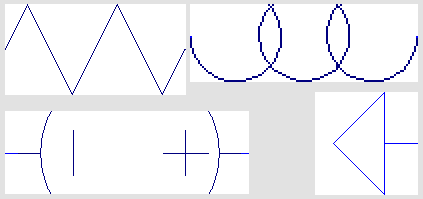
\includegraphics[width = 3.2in]{img/elements.png}
\caption{Examples of LTSpice-conform circuit elements}
\label{fig:c4}
\end{figure}

\subsection{Rectification}

To validate the rectification, 15 photographs of papers were collected and rectified. Then it was evaluated how many of the pixels that are not contained on the paper lay inside the rectified image. The average result is $99.5\%$, where the minimally measured value is $98.8\%$. The pixels that lay outside of the paper, that are contained in the rectified image, resulted from the paper not being flat on the ground resulting in small curls. Since the user has to select the area of the filter this proportion can be neglected.

\subsection{OCR}

To evaluate the OCR algorithm the number of detected text compared to the input image was calculated. 

\begin{table}[!ht]
\centering
\caption{Evaluation of OCR algorithm}
\label{tab:ocr}
\begin{tabular}{|l|l|l|}
\hline
Found w/o user & Found w/ user & Correct \\ \hline
73.62\%        & 100\%         & 95.7\%  \\ \hline
\end{tabular}
\end{table}

Instead of listing every single of the 30 tested images, only the average result is displayed in table \ref{tab:ocr}. The values that were evaluated is the text that was found without the user specifying a region, the text that was able to be detected and the amount of text that was correctly detected. The score of the found text without user interaction is somewhat low because the OCR algorithm supplied by MATLAB has trouble finding text if it is close to the components. Also, the correctly detected text is high, but the wrongly identified test is mostly caused by similar letters like upper- and lower case $P$.\\
Additionally, the same procedure was made for several images of two printed schematics. The text was always correctly detected, but the detection without user-interaction is $59.4\%$, which is expectedly lower compared to screenshots. This is due to noise in the image and a lower resolution.

\subsection{Scale Retrieval}

In order to evaluate the performance of the scale retrieval routine, the dimensions of the resistors of each image has been measured manually. Thereafter, each image was sent through the program until the resistor dimensions were retrieved. In table \ref{tab:resdim}, the dimensions of resistors in each image (column \textit{Measured}) can be found alongside the dimensions retrieved by the algorithm for each picture (column \textit{Calculated}) and a maximum deviance of the resistor size for each dimension. A manual measurement tolerance of one pixel is included in this maximum deviance metric.
\par

\begin{table}[H]
\centering
\begin{tabular}{l|l|l|l|l} \hline
		File & h/v & Measured & Calculated & Deviance\\ \hline \hline
		01.png & horiz. & $180\times91$ & $180\times88$ & $<1\times4$ \\ \hline
		02.png & vert. & $91\times180$ & $90\times194$ & $<2\times5$ \\ \hline
		03.png & horiz. & $180\times90$ & $176\times87$ & $<5\times4$ \\ \hline
		04.png & horiz. & $140\times71$ & $140\times69$ & $<1\times3$ \\ \hline
		05.png & vert. & $46\times92$ & $46\times96$ & $<1\times5$ \\ \hline
		06.png & vert. & $46\times92$ & $46\times96$ & $<1\times5$ \\ \hline
		07.png & horiz. & $206\times103$ & $208\times102$ & $<3\times2$ \\ \hline
		08.png & vert. & $108\times215$ & $106\times216$ & $<3\times2$ \\ \hline
		09.png & vert. & $85\times169$ & $83\times168$ & $<3\times2$ \\ \hline
		10.png & vert. & $127\times255$ & $126\times256$ & $<2\times2$ \\ \hline
		11.png & horiz. & $216\times108$ & $216\times107$ & $<1\times2$ \\ \hline
		12.png & vert. & $109\times216$ & $108\times212$ & $<2\times5$ \\ \hline
		13.png & horiz. & $199\times100$ & $200\times98$ & $<2\times3$ \\ \hline
		14.png & vert. & $94\times185$ & $91\times184$ & $<4\times2$ \\ \hline
		15.png & horiz. & $265\times133$ & $264\times130$ & $<2\times4$ \\ \hline
		16.png & horiz. & $215\times108$ & $216\times106$ & $<2\times3$ \\ \hline
		17.png & vert. & $98\times195$ & $94\times192$ & $<5\times4$ \\ \hline
		18.png & vert. & $108\times215$ & $108\times224$ & $<\textcolor[rgb]{0.8,0,0}{1\times10}$ \\ \hline
		19.png & vert. & $118\times235$ & $114\times232$ & $<5\times4$ \\ \hline
		20.png & horiz. & $245\times122$ & $248\times120$ & $<4\times3$ \\ \hline
\end{tabular}
\caption{Resistor size measurements and estimations (in px)}
\label{tab:resdim}
\end{table}
\par

A maximum deviance of 5 pixels is considered satisfactory for an effective usage of the object detection algorithm. With the exception of one case, the scale retrieval algorithm could retrieve the resistor size in all images it got called on. This corresponds to an accuracy of 95\%.

\subsection{Object Detection}

To evaluate the object detection algorithm, perfectly prepared images (screenshots of circuits without text) were used. The algorithm was tested on how well it detected all objects correctly and on the number of phantom detections, which are detections without actual objects being at concerned places.
\par
Through tables \ref{tab:det1} (collected data) and \ref{tab:det2} (main results), the following conclusions can be made:
\begin{itemize}
	\item There is a 4.8\% miss rate; The chance that an object is misclassified.
	\item There is a 3.9\% not-detection rate; The chance that an object is not recognized at all.
	\item There is a 7.4\% phantom rate; The chance that additional objects are recognized, where none actually are. This is in relation to total actual objects.
	\item The ratio between total number of candidates and total number of selected objects is 25\%, ranging from 13\% to 35\%.
	\item The correct identification rate, that is the number of correctly identified objects in relation to the number of actual present objects, is 90.9\%
\end{itemize}
\par

The detection algorithm performs well in certain circumstances. The detection algorithm has severe difficulties when the input images are not well rectified or cleaned (no text, no noise). The most common error sources were ground- or capacitor elements being recognized where none were, or where other sources were. This can be explained by their very simple and common shape. Voltage sources were also often misidentified or placed where no objects actually were (phantom objects).
\par

\begin{table}[H]
\centering
\begin{tabular}{l|l|l|l|l|l|l|l} \hline
		ID & EL & CC & SC & Cdet & Mdet & Ndet & Pdet \\ \hline \hline
		1&6&18&7&6&0&0&1\\ \hline
		2&6&17&6&6&0&0&0\\ \hline
		3&8&23&8&8&0&0&0\\ \hline
		4&9&22&10&9&0&0&1\\ \hline
		5&9&19&9&8&1&0&0\\ \hline
		6&11&26&11&10&1&0&0\\ \hline
		7&8&18&8&8&0&0&0\\ \hline
		8&5&24&5&5&0&0&0\\ \hline
		9&11&35&12&11&0&0&1\\ \hline
		10&7&13&7&7&0&0&0\\ \hline
		11&8&24&9&8&0&0&1\\ \hline
		12&6&35&5&4&0&2&1\\ \hline
		13&5&15&6&5&0&0&1\\ \hline
		14&7&21&9&6&1&0&2\\ \hline
		15&7&17&6&6&0&1&0\\ \hline
		16&6&22&7&5&0&1&2\\ \hline
		17&9&25&10&9&0&0&1\\ \hline
		18&7&28&7&6&0&1&1\\ \hline
		19&7&24&7&6&0&1&1\\ \hline
		20&7&22&6&5&0&2&1\\ \hline
		21&9&24&10&9&0&0&1\\ \hline
		22&8&30&9&7&1&0&0\\ \hline
		23&9&25&9&9&0&0&0\\ \hline
		24&7&13&7&6&1&0&0\\ \hline
		25&9&36&9&8&1&0&0\\ \hline
		26&7&32&10&6&1&0&2\\ \hline
		27&8&29&7&7&0&1&0\\ \hline
		28&8&36&8&6&2&0&0\\ \hline
		29&7&28&7&6&1&0&0\\ \hline
		30&8&29&8&7&1&0&0\\ \hline \hline
			& REL & & & & 4.8\% & 3.9\% & 7.4\% \\ \hline
\end{tabular}
\caption{Collected data from tests. ID: Test image ID, EL: Nr. of correct elements, CC: Candidate Count, SC: Selected Count, Cdet: Correctly detected, Mdet: Misdetected, Ndet: Not detected, Pdet: Phantom detected}
\label{tab:det1}
\end{table}
\par

\begin{table}[H]
\centering
\begin{tabular}{l|l|l|l} \hline
		ID & SR\% & ELEM & CORR\% \\ \hline \hline
		1&28\%&6&100\%\\ \hline
		2&26\%&6&100\%\\ \hline
		3&26\%&8&100\%\\ \hline
		4&31\%&9&100\%\\ \hline
		5&32\%&9&89\%\\ \hline
		6&30\%&11&91\%\\ \hline
		7&31\%&8&100\%\\ \hline
		8&17\%&5&100\%\\ \hline
		9&26\%&11&100\%\\ \hline
		10&35\%&7&100\%\\ \hline
		11&27\%&8&100\%\\ \hline
		12&13\%&6&67\%\\ \hline
		13&29\%&5&100\%\\ \hline
		14&30\%&7&86\%\\ \hline
		15&26\%&7&86\%\\ \hline
		16&24\%&6&83\%\\ \hline
		17&29\%&9&100\%\\ \hline
		18&20\%&7&86\%\\ \hline
		19&23\%&7&86\%\\ \hline
		20&21\%&7&71\%\\ \hline
		21&29\%&9&100\%\\ \hline
		22&23\%&8&88\%\\ \hline
		23&26\%&9&100\%\\ \hline
		24&35\%&7&86\%\\ \hline
		25&20\%&9&89\%\\ \hline
		26&24\%&7&86\%\\ \hline
		27&19\%&8&88\%\\ \hline
		28&18\%&8&75\%\\ \hline
		29&20\%&7&86\%\\ \hline
		30&22\%&8&88\%\\ \hline \hline
		Avg & 25\% & & 90.9\%\\ \hline
\end{tabular}
\caption{Caption: Results of evaluation. ID: Test image ID, SR\%: Selected Ratio, ELEM: Nr. of correct elements, CORR\%: Correct ratio}
\label{tab:det2}
\end{table}
\par

% CONCLUSION----------------------------------------------------

\section{Conclusion}

This paper introduced a method to digitalize electrical circuits given in form of an image, using a sliding-window approach for the detection of the electrical elements of the circuit. Despite the staticness of this approach, using certain assumptions concerning the appearance of the circuit and its parts, the algorithm produced exact models and accurate topographies in a relatively stable manner.

\subsection*{Ideas for future work}

Despite promising results, there are several measures which could improve this work:
\begin{itemize}
	\item A limiting factor of this approach, especially when dealing with photographies, was the detection of lines using MATLAB's hough transformation implementation. Implementing a new and custom hough transformation is a promising way to make the retrieval of connections more robust. \textbf{Additionally, this resulted in lines not being detected after the rectification, which explains why this part was not validated TODO}.
	\item Similar to MATLAB's hough transform, its OCR functionality also struggled to correctly and robustly detect the text in the test schematics. A proper OCR solution would increase the robustness of the whole procedure just like an improved hough transform would.
	\item Within the object detection, instead of the comparison of image regions with the respective templates and the following calculation of error images, the process of finding electrical elements could be made more abstract, e.g. by comparing histograms of geometrical primitive imformations such as line length and angle instead of comparing color values pixel by pixel. Such an abstraction can potentially increase the tolerance of the object detection algorithm regarding the deviance of the found circuit elements from the template.
\end{itemize}

% CONTRIB-------------------------------------------------------

\section*{Contributions}
\label{sec:contrib}

\begin{table}[H]
\centering
\begin{tabular}{l|l l l} \hline
		Name & Proposal & Research & Pres.\\ \hline
		Andreas Boltres & 25\% & 25\% & 25\% \\
		Cem G\"ul\c{s}an & 25\% & 25\% & 25\% \\
		Christian Vecsei & 25\% & 25\% & 25\% \\
		Thomas Frei & 25\% & 25\% & 25\%  \\ \hline
		& 100\% & 100\% & 100\% \\ \hline \hline
		     & Paper & Spirit & Candy\\ \hline
		Andreas Boltres & 25\% & 25\% & 25\% \\
		Cem G\"ul\c{s}an & 25\% & 25\% & 25\% \\
		Christian Vecsei & 25\% & 25\% & 25\% \\
		Thomas Frei & 25\% & 25\% & 25\% \\ \hline
		& 100\% & 100\% & 100\% \\ \hline
\end{tabular}
\caption{List of members and their contributions to the project.}
\label{tab:contrib}
\end{table}

\end{document}
